\documentclass[]{article}
\usepackage{lmodern}
\usepackage{amssymb,amsmath}
\usepackage{ifxetex,ifluatex}
\usepackage{fixltx2e} % provides \textsubscript
\ifnum 0\ifxetex 1\fi\ifluatex 1\fi=0 % if pdftex
  \usepackage[T1]{fontenc}
  \usepackage[utf8]{inputenc}
\else % if luatex or xelatex
  \ifxetex
    \usepackage{mathspec}
  \else
    \usepackage{fontspec}
  \fi
  \defaultfontfeatures{Ligatures=TeX,Scale=MatchLowercase}
\fi
% use upquote if available, for straight quotes in verbatim environments
\IfFileExists{upquote.sty}{\usepackage{upquote}}{}
% use microtype if available
\IfFileExists{microtype.sty}{%
\usepackage{microtype}
\UseMicrotypeSet[protrusion]{basicmath} % disable protrusion for tt fonts
}{}
\usepackage[unicode=true]{hyperref}
\hypersetup{
            pdftitle={Design Document - v1.0},
            pdfauthor={Gianpaolo Branca; Luca Butera; Andrea Cini},
            pdfborder={0 0 0},
            breaklinks=true}
\urlstyle{same}  % don't use monospace font for urls
\usepackage{graphicx,grffile}
\makeatletter
\def\maxwidth{\ifdim\Gin@nat@width>\linewidth\linewidth\else\Gin@nat@width\fi}
\def\maxheight{\ifdim\Gin@nat@height>\textheight\textheight\else\Gin@nat@height\fi}
\makeatother
% Scale images if necessary, so that they will not overflow the page
% margins by default, and it is still possible to overwrite the defaults
% using explicit options in \includegraphics[width, height, ...]{}
\setkeys{Gin}{width=\maxwidth,height=\maxheight,keepaspectratio}
\IfFileExists{parskip.sty}{%
\usepackage{parskip}
}{% else
\setlength{\parindent}{0pt}
\setlength{\parskip}{6pt plus 2pt minus 1pt}
}
\setlength{\emergencystretch}{3em}  % prevent overfull lines
\providecommand{\tightlist}{%
  \setlength{\itemsep}{0pt}\setlength{\parskip}{0pt}}
\setcounter{secnumdepth}{0}
% Redefines (sub)paragraphs to behave more like sections
\ifx\paragraph\undefined\else
\let\oldparagraph\paragraph
\renewcommand{\paragraph}[1]{\oldparagraph{#1}\mbox{}}
\fi
\ifx\subparagraph\undefined\else
\let\oldsubparagraph\subparagraph
\renewcommand{\subparagraph}[1]{\oldsubparagraph{#1}\mbox{}}
\fi

% set default figure placement to htbp
\makeatletter
\def\fps@figure{htbp}
\makeatother


\title{\textbf{Design Document - v1.0}}
\author{Gianpaolo Branca \and Luca Butera \and Andrea Cini \newline}
\date{
\includegraphics{polimi.png}\newpage}

\begin{document}
\maketitle

{
\setcounter{tocdepth}{3}
\tableofcontents
}
\newpage

\section{Introduction}\label{introduction}

\subsection{Purpose}\label{purpose}

The purpose of this document is to provide technical informations about
the service we are going to deploy described in the RASD.

\subsection{Scope}\label{scope}

Our service is about electric car sharing to provide a valid option to
public transportation for low length trips. It is provided via mobile
application for the final users and via web application for the
operators of the company. Users can download the app with the Android
play store or with the Apple store. Operators can enter the system
directly from a browser in the boundaries of the companies network after
logging in.

\subsection{Definitions, Acronyms,
Abbreviations}\label{definitions-acronyms-abbreviations}

\begin{itemize}
\tightlist
\item
  PWE: PoWer Enjoy.
\item
  API: application programming interface, in this document we are mainly
  referring to web APIs that are defined interfaces through which the
  client-server interaction happens.
\item
  QR code: a matrix barcode.
\item
  JEE : Java Enterprise Edition, a set of APIs and a runtime environment
  for developing and running enterprise software.
\item
  RESTful: REpresentational State Transfer web services provide
  interoperability between computer systems on the net allowing the
  client-server interaction through a set of pre-defined stateless
  operations.
\item
  JAX-RS: Java API for RESTful Services, the Java APIs for developing
  RESTful compliant applications, JAX-RS is part of the JEE framework.
\item
  JDBC: Java DataBase Connection, a set of Java APIs which defines the
  interaction between a Java program and a DBMS JDBC compatible.
\item
  DBMS: DataBase Management System, a software system to handle the
  creation, the manipulation and the retrieval of data in a database.
\item
  JSON: JavaScript Object Notation, it's a lightweight format for
  data-interchange.
\item
  RASD: Requirements Analysis and Specification Document.
\item
  DD: Design Document.
\item
  Legacy system: the already existing system of the company
\item
  Ride: with ride we refer to the set of operations that begin with the
  user checking-in in the car and that end with the user checking-out.
\item
  TLS: Transport layer security, cryptographic protocol tha grants
  security over a computer network.
\end{itemize}

\subsection{Reference documents}\label{reference-documents}

\begin{itemize}
\tightlist
\item
  RASD
\item
  Specification document \newpage
\end{itemize}

\section{Architectural Design}\label{architectural-design}

\subsection{Overview}\label{overview}

We are going to build our system following these guidelines (appropriate
reasons for each choice will be given in the next sections):

\begin{enumerate}
\def\labelenumi{\arabic{enumi}.}
\item
  Our application will be implemented using a three-tier architecture
  for each application, as it is the most suitable(this point will be
  clear in the next steps) and maintainable one for our system.
\item
  For the mobile application the client side will be light-weighted,
  with only the presentation layer as there's no need to perform any
  kind of data manipulation on the user's mobile phone.
\item
  The car will be equipped with a machine with our application running
  on it. On the contrary of the mobile app case, the on-board
  application will need to exploit some logic to perform its
  functionalities.
\item
  The operators will access the system through a web application.
\item
  Integration with the legacy server will happen trough its APIs for the
  purpose of providing maintenance to the cars and clients care.
\item
  Firewalls will keep secure the communications with the mobile clients
  and the cars.
\end{enumerate}

Refer to the Architectural and technological choices for a more in depth
analysis of this points.

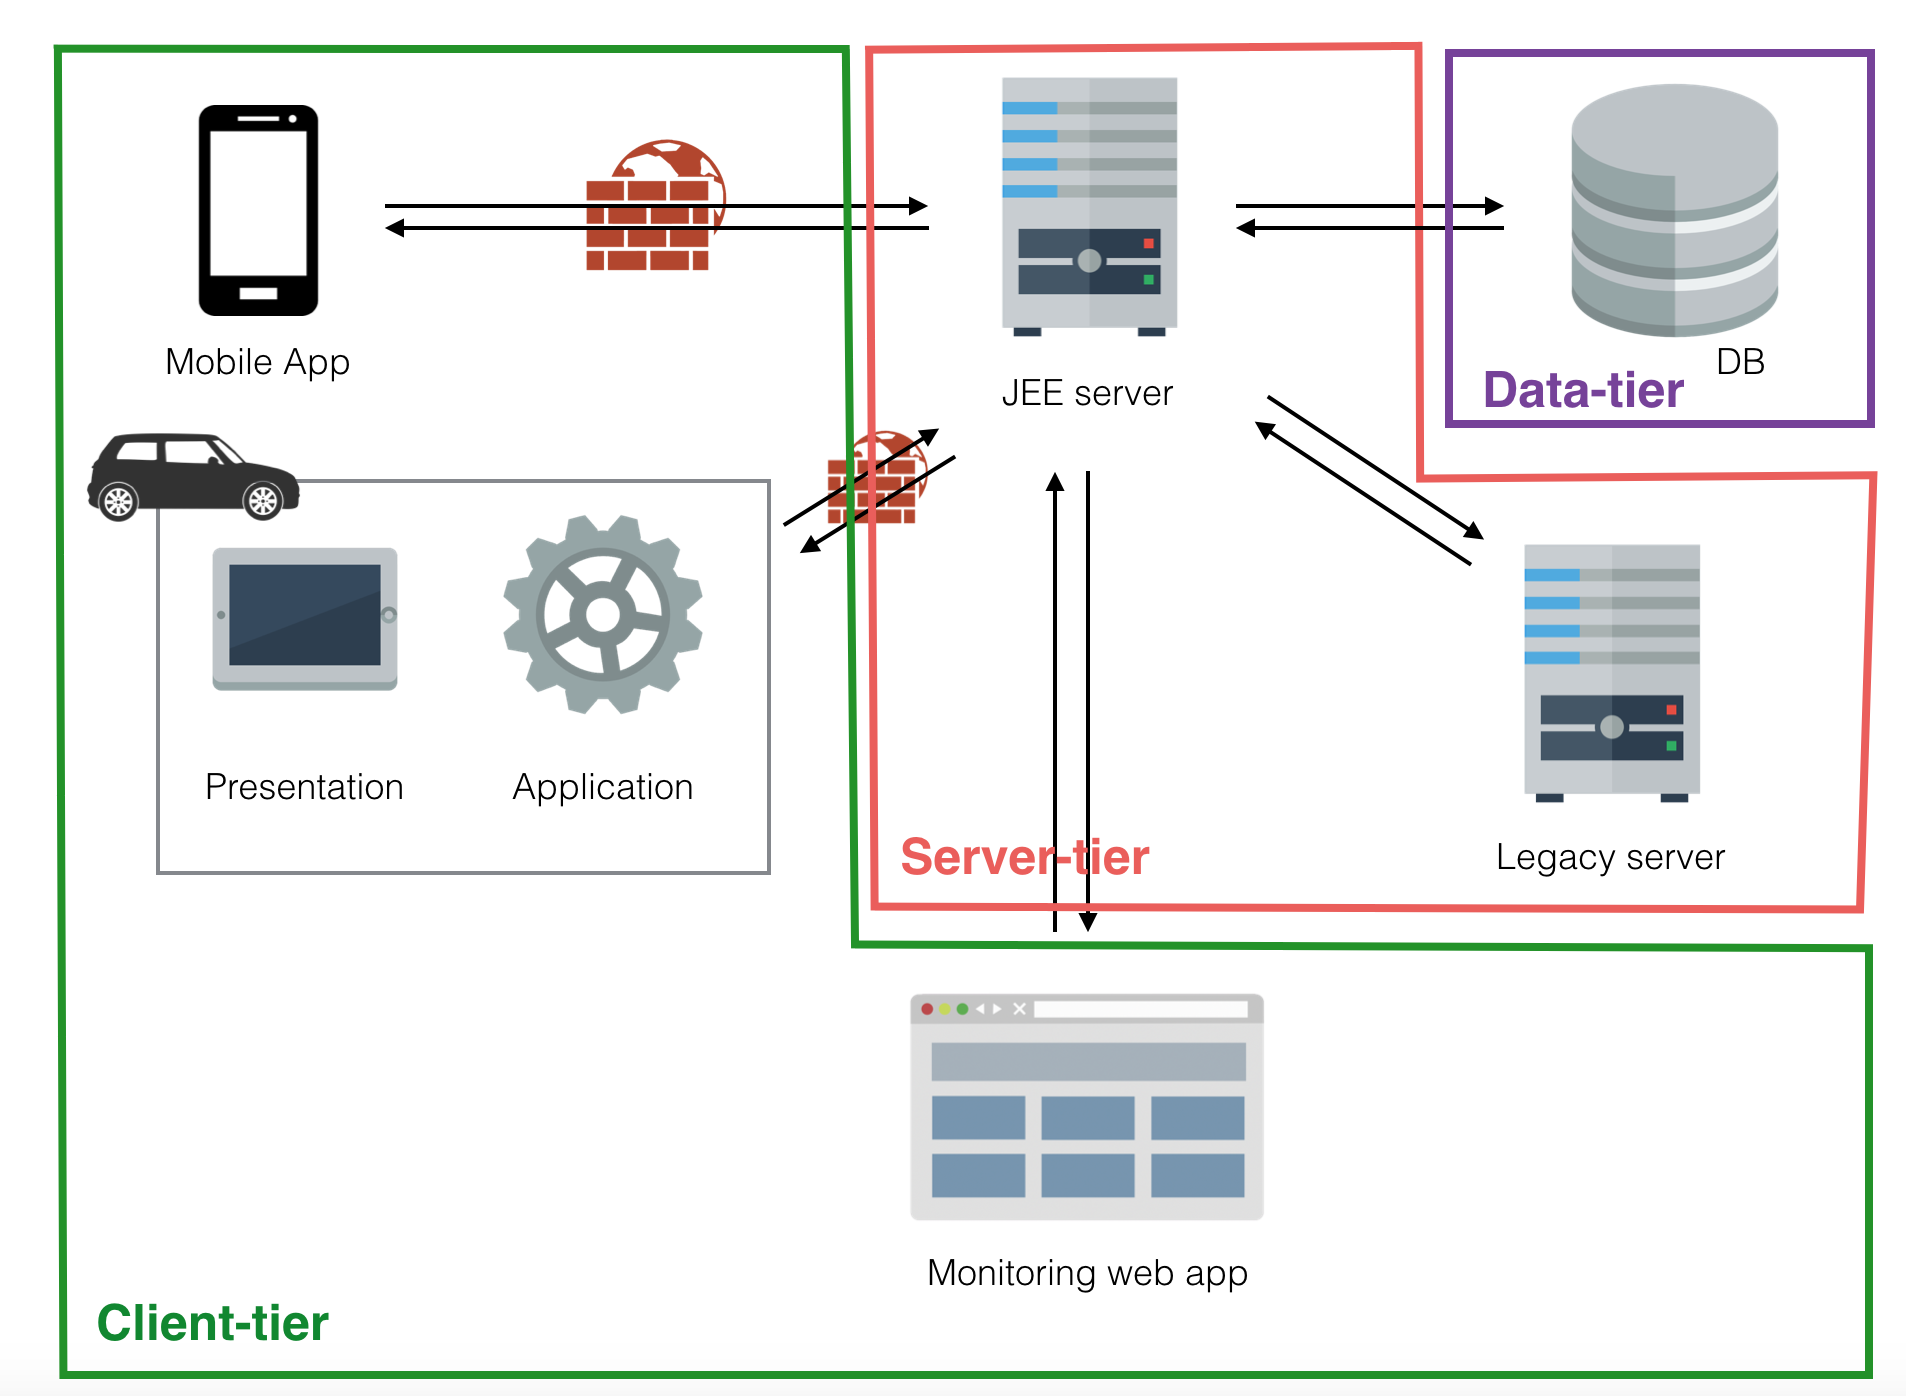
\includegraphics[width=1.00000\textwidth,height=1.00000\textwidth]{./images/sysApp.png}
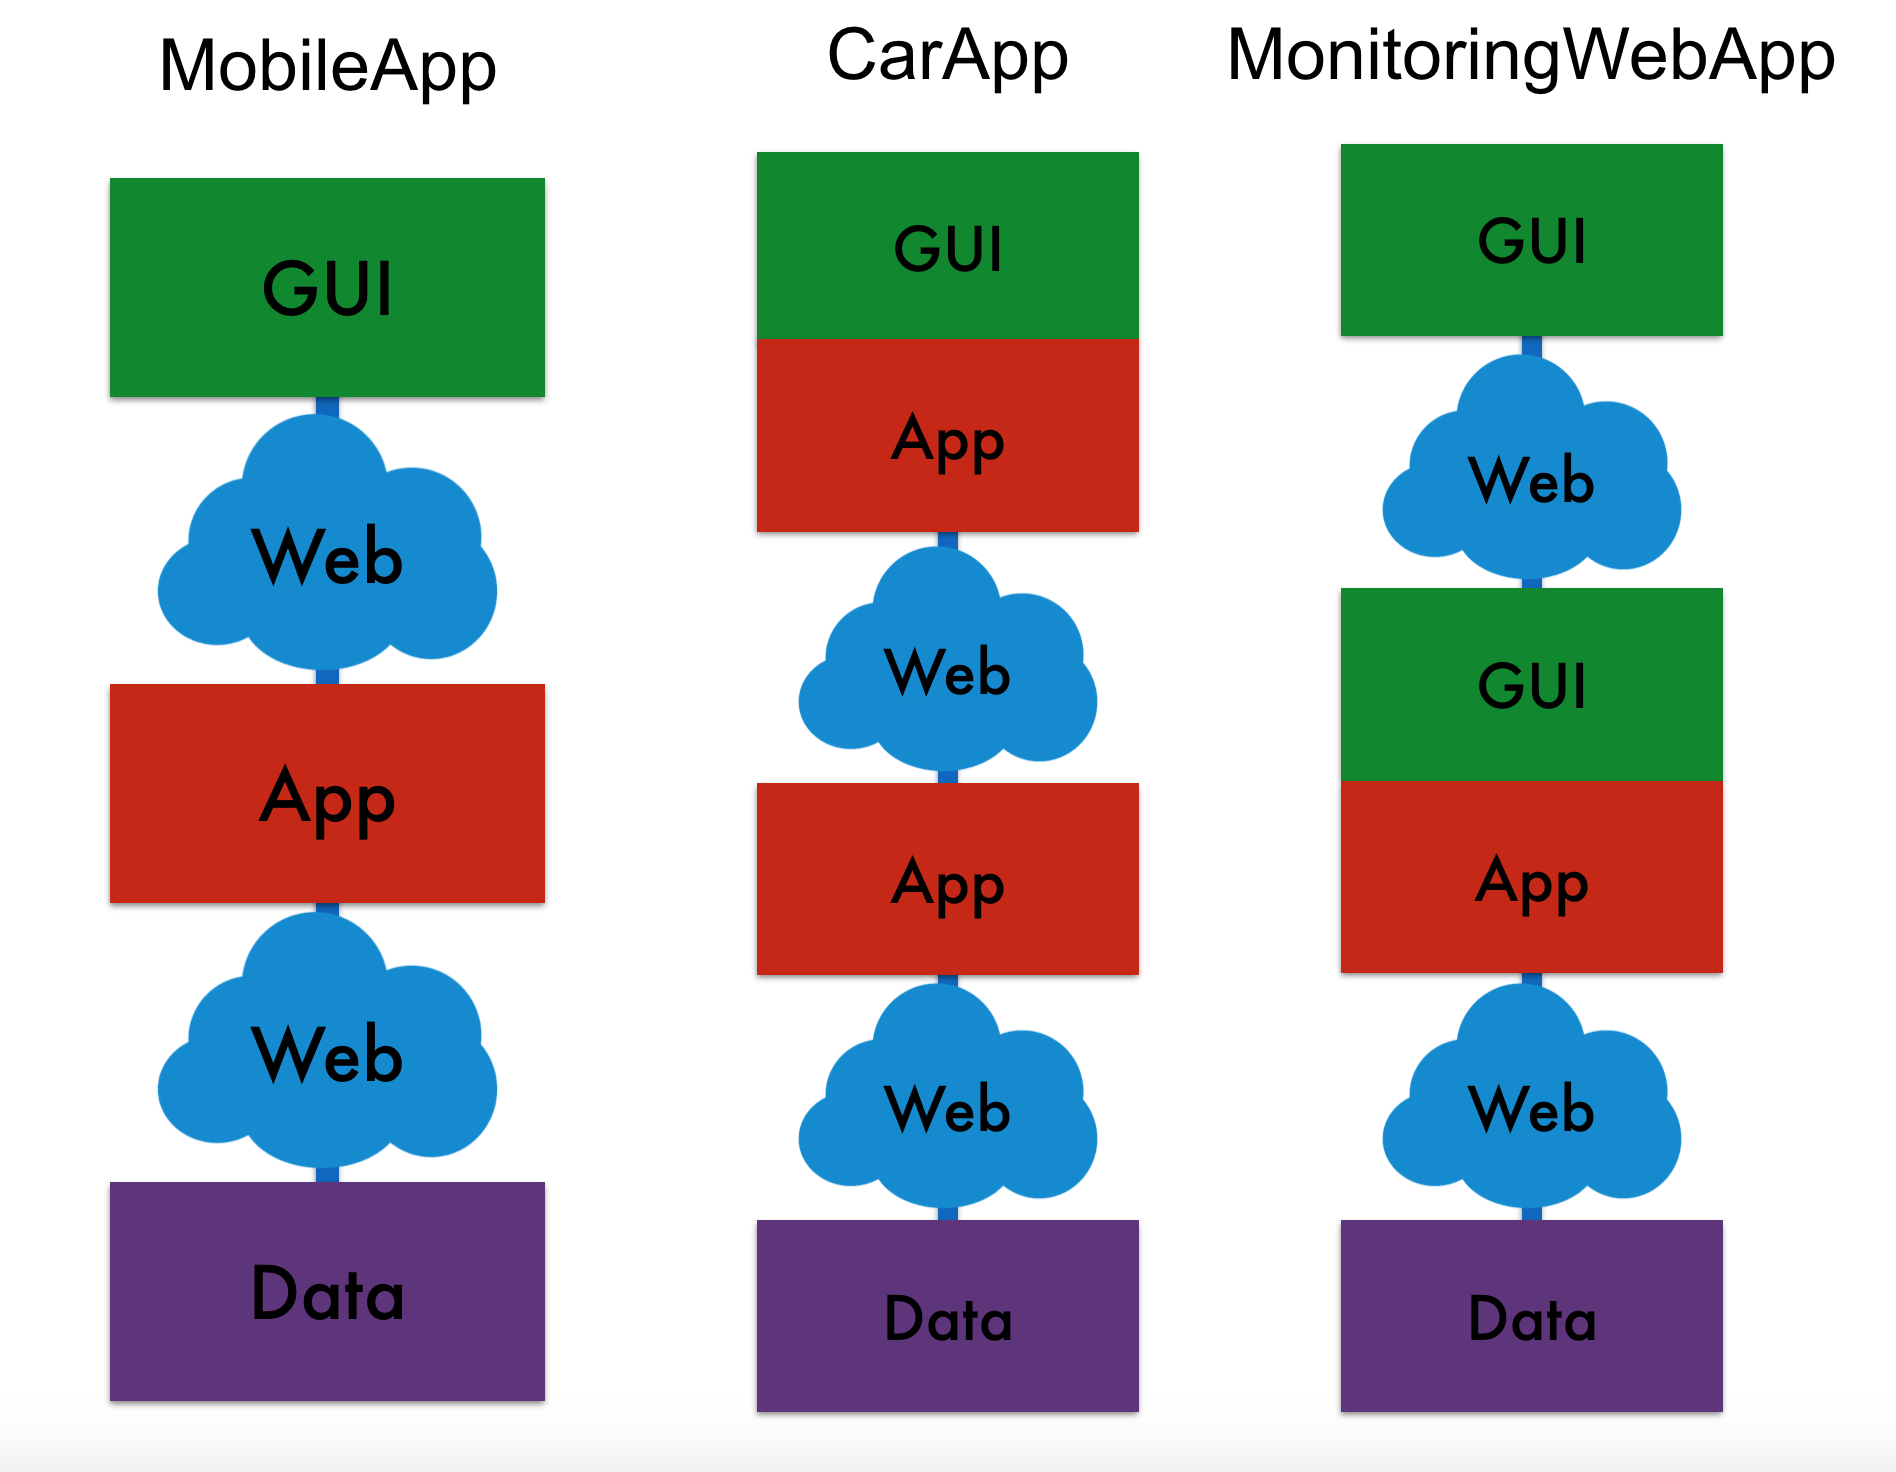
\includegraphics[width=1.00000\textwidth,height=1.00000\textwidth]{./images/layers.png}

\subsection{High level component view}\label{high-level-component-view}

In this section we are going to give a look at the architectural
structure of our system at the level of the components that we are going
to develop and the main ones that we are going to interact with.
\newline

\begin{figure}
\centering
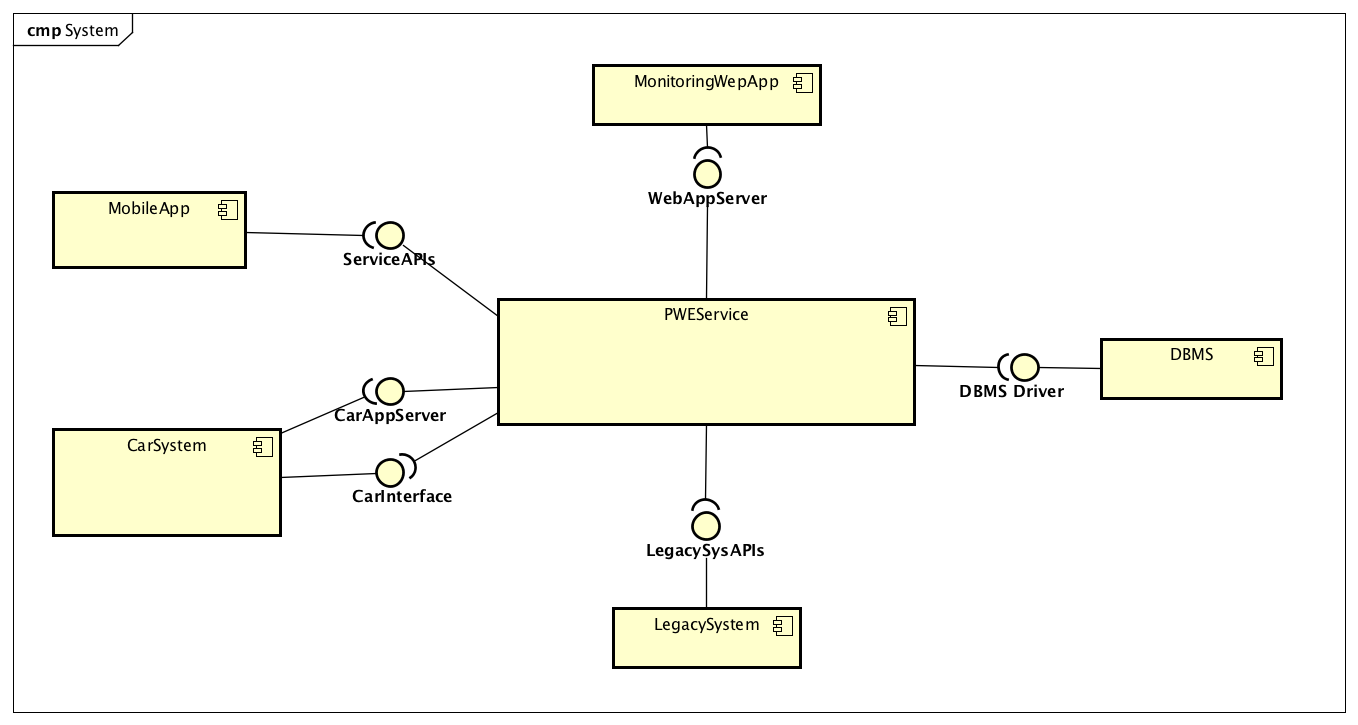
\includegraphics[width=1.00000\textwidth,height=1.00000\textwidth]{./comp_diagrams/System.png}
\caption{}\label{id}
\end{figure}

Components to be developed:

\begin{itemize}
\tightlist
\item
  \textbf{PWEService}: It is the core of the system, it has a role of
  services provider and tasks coordinator. The core of the logic aimed
  to fulfill our business goals is implemented here.
\item
  \textbf{CarSystem}: The component representing the on-board
  application of the car, its main functionalities are the ones related
  to the handling of a ride and the monitoring of the car status. It
  also offers presentation functionalities to give(receive) feedback
  to(from) the client. It expose its own interface to grant the central
  component control over its functionalities and uses a dedicated
  PWEInterface to ask for the server services and to send updates.
\item
  \textbf{MobileApp}: The component providing the client the access to
  the system. It fulfills only presentation functions. It behaves like a
  synchronous client and interacts with the central component through
  the ServiceAPIs in a call/response, classic client-server fashion.
\item
  \textbf{MonitoringWebApp}: The component providing operators of the
  company access to monitoring and configuration functionalities. It has
  only presentation functionalities(web pages) and communicates with the
  central component through the provided interface.
\end{itemize}

Components to be integrated in the system:

\begin{itemize}
\tightlist
\item
  \textbf{LegacySystem}: the already existing system of the company, our
  system will exploit its functionalities through the provided APIs.
\item
  \textbf{DBMS}: the system that will take care of the management of our
  data, integrated in our system using a specific driver.
\item
  \textbf{GoogleMaps and PayPal}: respectively the provider of the maps
  and the payment service(they are not in the diagram, their integration
  in the system will be discussed later on).
\end{itemize}

\subsection{Component view}\label{component-view}

\paragraph{Car System}\label{car-system}

\begin{figure}
\centering
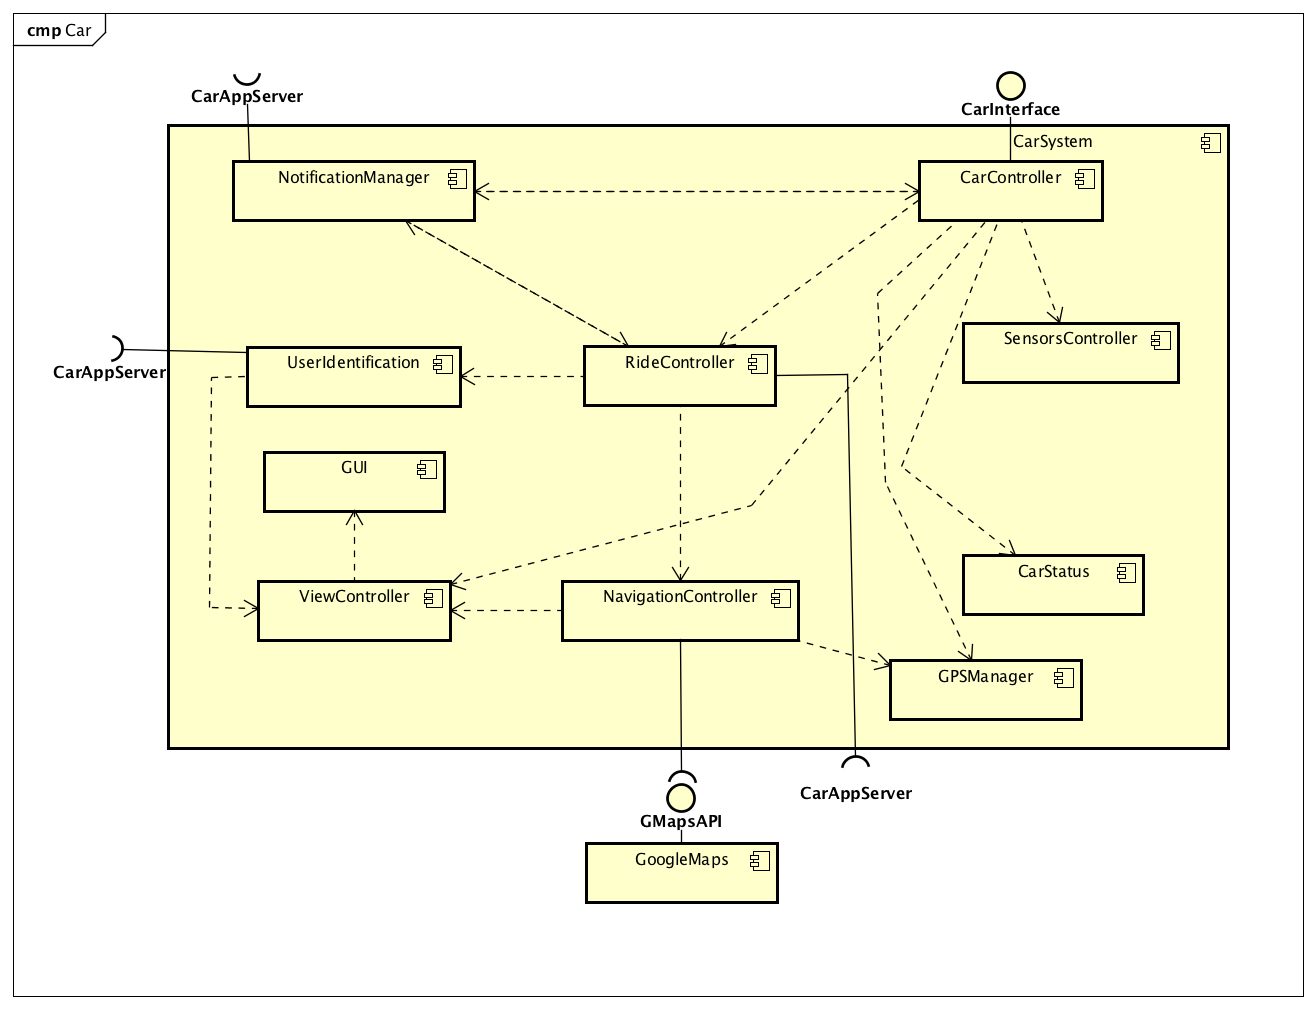
\includegraphics[width=1.00000\textwidth,height=1.00000\textwidth]{./comp_diagrams/CarSystem.png}
\caption{}\label{id}
\end{figure}

Components description:

\begin{itemize}
\tightlist
\item
  \textbf{CarController} : The main controller of the car. It retrieves
  informations from the other components, executes the requests of the
  server and updates the car status.
\item
  \textbf{RideController} : The handler of the operations concerning the
  execution of a ride. It communicates with the central component which
  has its own control functionalities over the ride: after the users
  have been identified the ride controller creates the ride instance,
  communicates the initial details on the ride to the central system
  (e.g.~the number of passengers) and then goes on sending updates
  periodically or when the ride status change (e.g.~the car exits the
  city boundaries), further details will be given in the runtime view.
\item
  \textbf{UserIdentification} : The component that will handle the
  identification of the users that check-in at the start of the ride.
\item
  \textbf{Navigation Controller} : The component that will provide
  navigation utilities using the GoogleMaps APIs and the GPS.
\item
  \textbf{GPSManager} : The component that will handle GPS localization
  of the car.
\item
  \textbf{CarStatus} : An internal representation of the status of the
  car.
\item
  \textbf{SensorsController}: The component that handles the retrieval
  of information from the sensors thought the OBD interface.
\item
  \textbf{NotificationManager}: The component that handles notifications
  coming from the central component and that perform the sending of the
  outgoing ones.
\item
  \textbf{ViewControlLer}: The component that handles the update of the
  GUI and the retrieval of the user input through the interface.
\item
  \textbf{GUI}: Implementation of the presentation layer of the car
  application. \newpage
\end{itemize}

\paragraph{PWEService and Model}\label{pweservice-and-model}

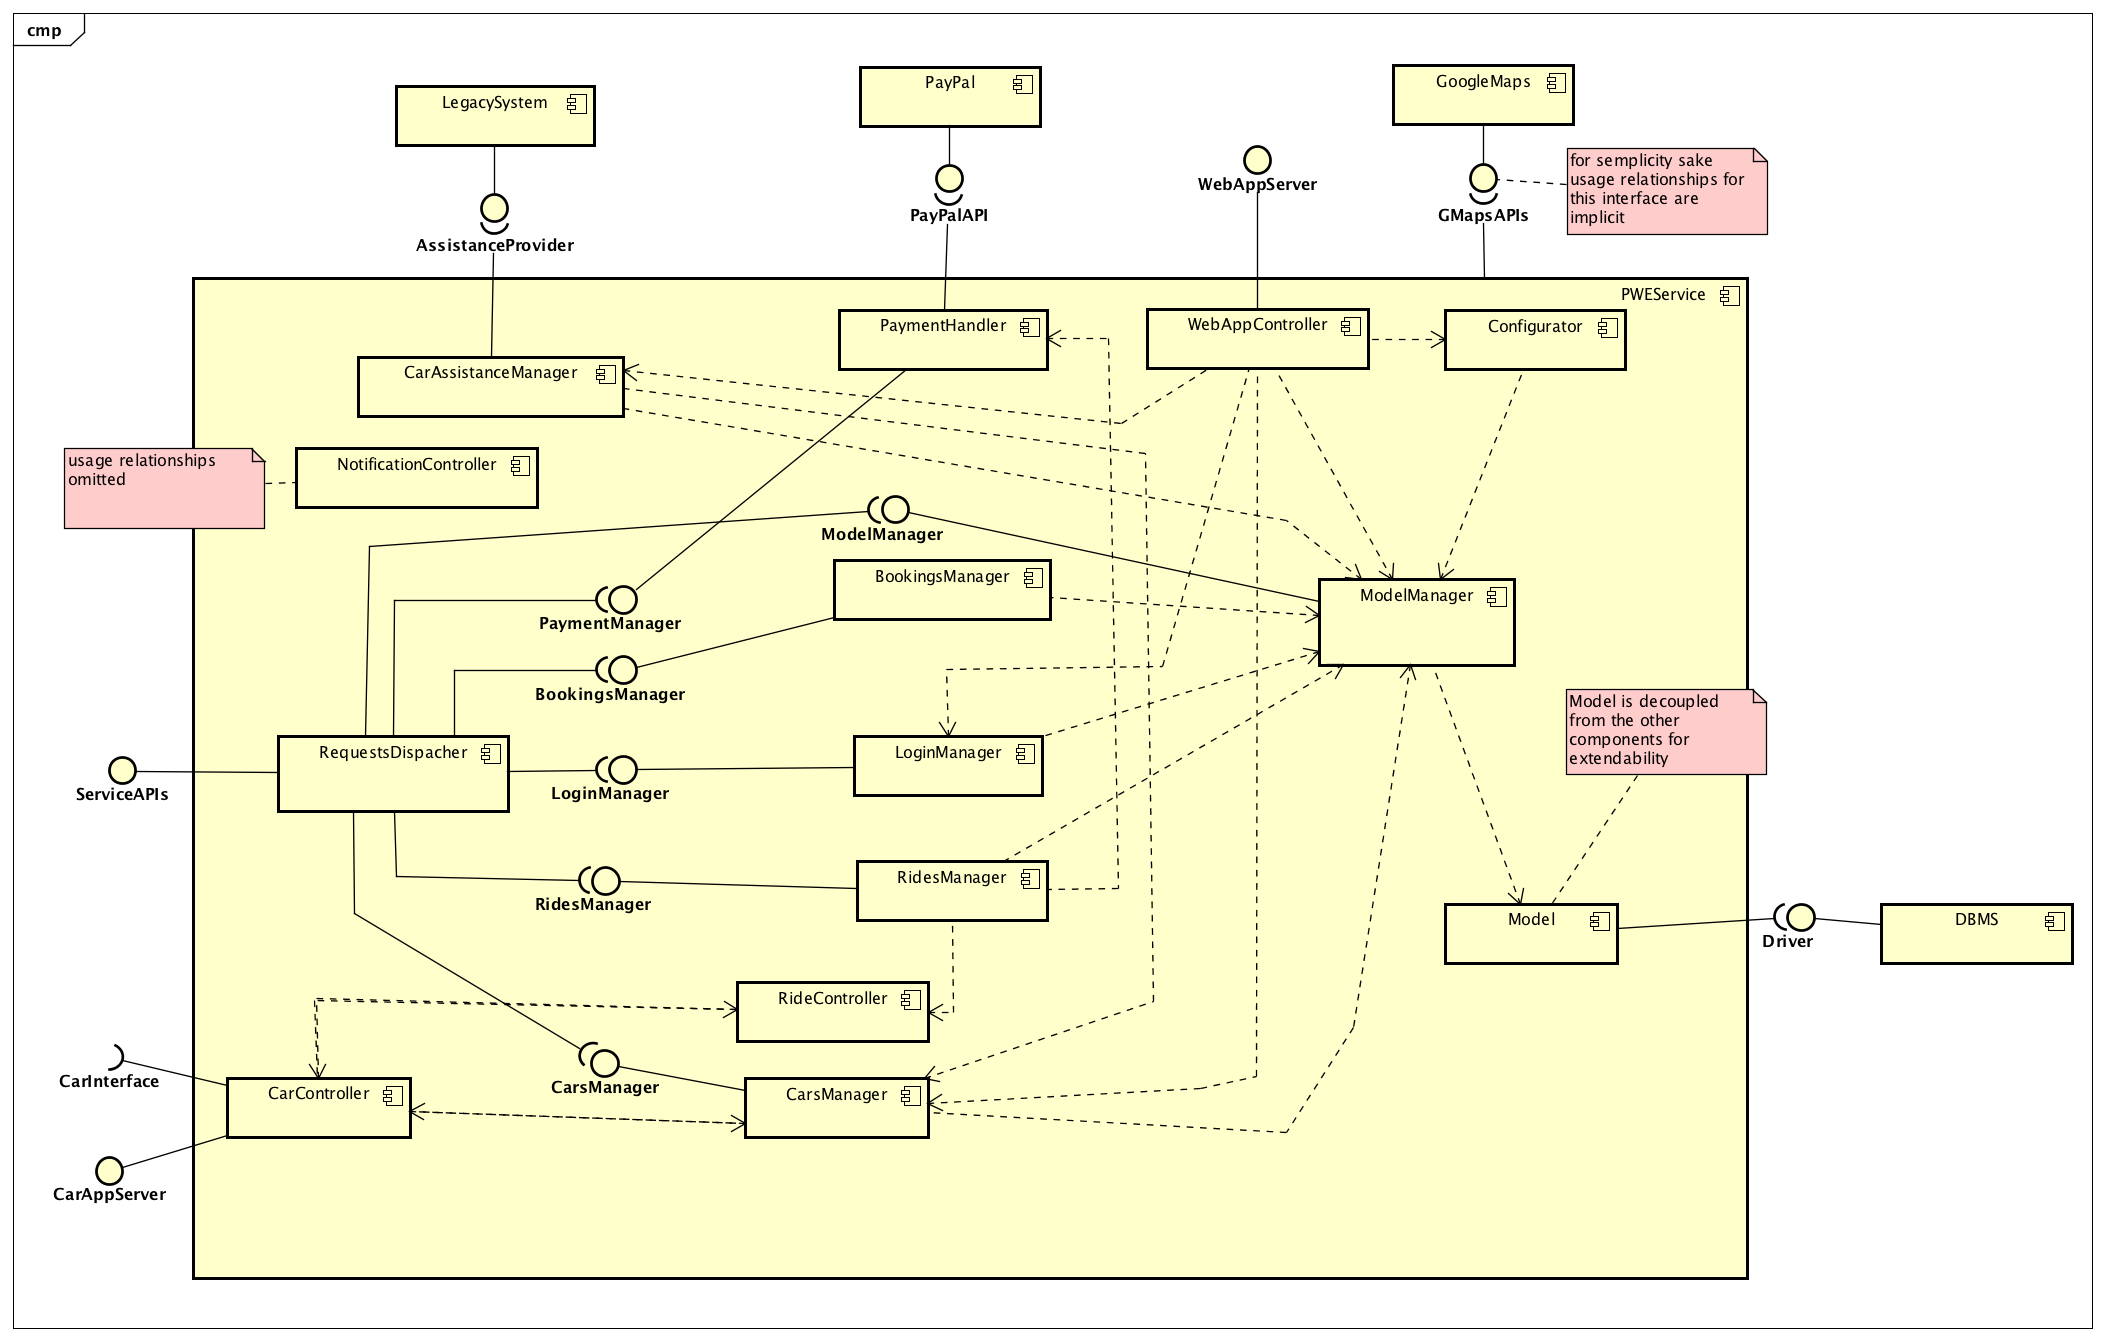
\includegraphics[width=1.00000\textwidth,height=1.00000\textwidth]{./comp_diagrams/PWEService.png}
\newline

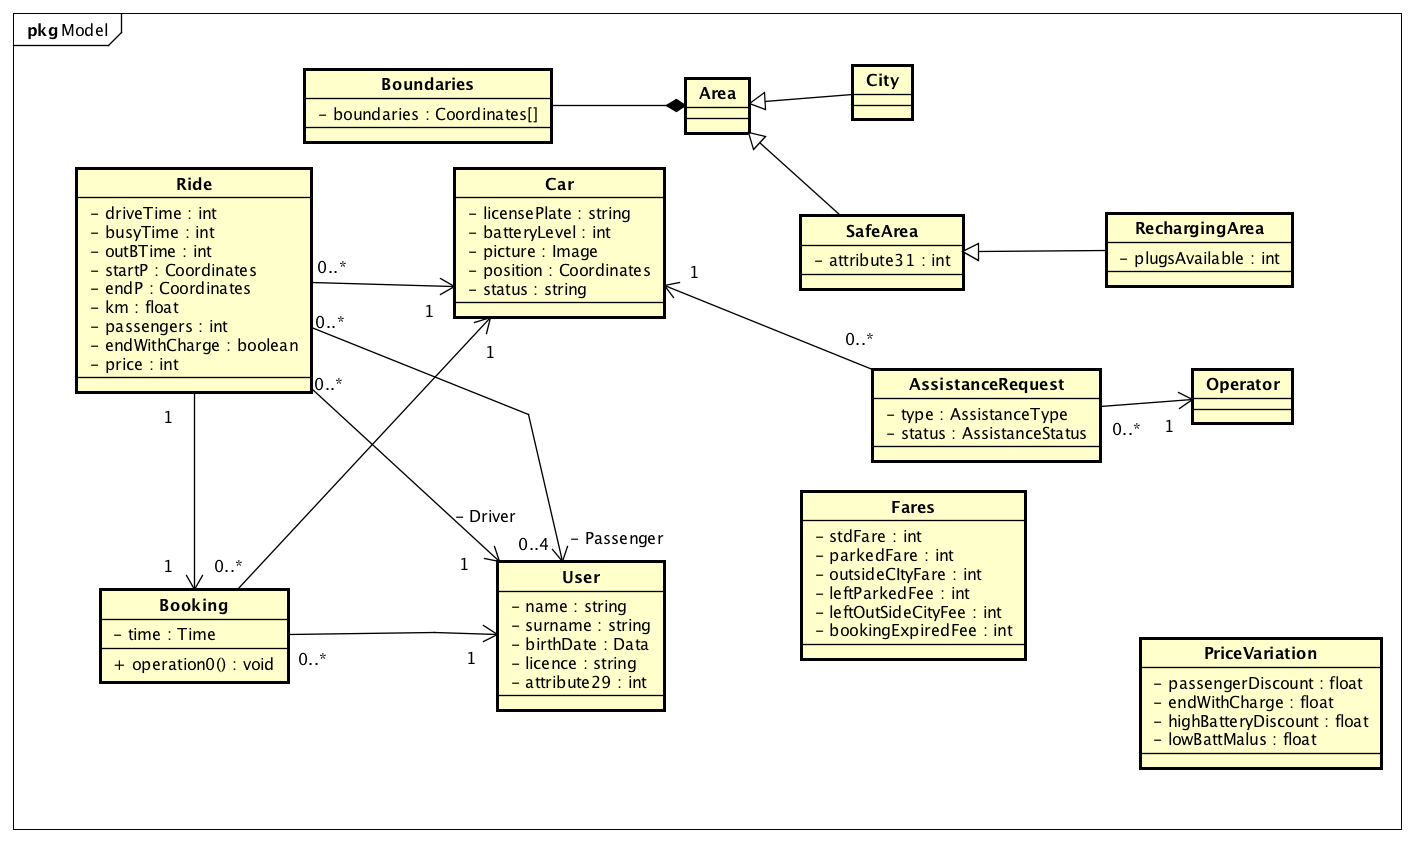
\includegraphics[width=1.00000\textwidth,height=1.00000\textwidth]{./comp_diagrams/Model.png}
\newline

Components description:

\begin{itemize}
\tightlist
\item
  \textbf{RequestDispatcher}: The component handles the requests from
  the mobile application clients using the functionalities of the
  specific components and sends back the responses.
\item
  \textbf{BookingManager}: The component that handles the operations
  concerning the usage of a car.
\item
  \textbf{RideController}: It interacts with the RideController
  component in the car as already mentioned in the section above the way
  the two components interact with each other will be clarified in the
  Runtime View section.
\item
  \textbf{RidesManager}: The component that handles the set of rides
  that are ongoing in the system, it interacts with the other components
  to give the single RideController access to the functionalities that
  it needs.
\item
  \textbf{CarController}: It interacts with the CarController component
  in the single car to offer services and perform supervising
  functionalities over a single vehicle.
\item
  \textbf{CarsManager}: The component the supervises the set of all the
  car available in the system interacting with the single CarController
  and providing operators with informations about the cars status and a
  way to change the status itself.
\item
  \textbf{LoginManager}: The component that handles the log-in of
  operators and users.
\item
  \textbf{PaymentHandler}: The component that handles the payment
  operations and makes sure that users unable to pay are correctly
  banned until they pay. It uses the PayPal APIs to process the
  payments.
\item
  \textbf{PayPal}: The payment handler of choice for our system.
\item
  \textbf{LegacySystem}: The old system of the company, our system uses
  its APIs to send assistance where needed.
\item
  \textbf{CarAssistanceManager}: The component that offers the
  functionalities needed to provide assistance to the vehicle when they
  need to moved, recharged or repaired. It exploits the functionalities
  of the legacy system to send road-operators to the car location.
\item
  \textbf{WebAppController}: The component the makes the system
  functionalities accessible from the WebApplication.
\item
  \textbf{Configurator}: The component that offers the configuration
  functionalities to customize a set of parameters of the system (set of
  SafeAreas, fares, fees and so on).
\item
  \textbf{NotificationController}: a component that offers notification
  functionalities towards the various components of the system.
\item
  \textbf{Model}: the structure of the data in our system (specified in
  a distinct diagram).
\item
  \textbf{GoogleMaps}: Provider of the maps services.
\end{itemize}

\subsection{Requirements Traceability}\label{requirements-traceability}

In this section we will show how the components of our system are meant
to satisfy the requirement and goals specified in the RASD. For utility
we report the goals and requirements here too.

\subsubsection{Goals}\label{goals}

The system must:

\begin{itemize}
\tightlist
\item
  {[}G0{]} Make the user able to access to the system.
\item
  {[}G1{]} Allow the clients to find an available car within a selected
  radius around his or a specified location.
\item
  {[}G2{]} Allow the clients to book a car and pick it up.
\item
  {[}G3{]} Monitor the usage of the car and charge the client with the
  right fare.
\item
  {[}G4{]} Incentivize a correct usage of the service to allow as many
  as possible users to use the same car without the need of the service
  of an operator.
\item
  {[}G5{]} Ensure a correct distribution of cars in the recharging
  stations according to the available plugs.
\item
  {[}G6{]} Allow operators to manage and monitor the state of all the
  cars and notify them when maintenance is needed on a specific vehicle.
\item
  {[}G7{]} Allow management system to set up and modify parameters of
  the system.
\item
  {[}G8{]} Provide a real time, interactive, pleasant and transparent
  user experience.
\end{itemize}

\subsubsection{Functional Requirements}\label{functional-requirements}

In the following section we are going to identify the requirements that
our system will have to fulfill to reach the goals.

\begin{itemize}
\item
  {[}G0{]} Make the user able to access to the system.

  \begin{itemize}
  \tightlist
  \item
    {[}R0.1{]} A user must sign up with valid credential.
  \item
    {[}R0.2{]} The system must generate a password for the user and send
    it to him through e-mail.
  \item
    {[}R0.3{]} A user must be able to visualize and modify all his
    personal informations.
  \end{itemize}
\item
  {[}G1{]} Allow the clients to find an available car within a selected
  radius around his or a specified location.

  \begin{itemize}
  \tightlist
  \item
    {[}R1.1{]} The system must be able to retrieve the location of the
    user.
  \item
    {[}R1.2{]} The user must be able to scroll the map of the city to
    find a car or specify the radius (in km) around a selected location
    for the car research.
  \item
    {[}R1.3{]} Upon the selection of a car the system must show an
    informative screen with current car details.
  \end{itemize}
\item
  {[}G2{]} Allow the clients to book a car and pick it up.

  \begin{itemize}
  \tightlist
  \item
    {[}R2.1{]} A client must be able to choose one of the available cars
    and book it.
  \item
    {[}R2.2{]} Once a car has been booked no others reservation can be
    performed by the same client until the first one is pending.
  \item
    {[}R2.3{]} After the reservation has been confirmed to the client,
    he has a maximum of 1 hour to reach the car, unlock it and start the
    engine. If the timeout expires the reservation is cancelled and a
    fee is applied.
  \item
    {[}R2.4{]} The user is able to unlock a booked car trough the app at
    any time after the reservation, however he has a maximum of 15
    minutes to turn it on after the unlocking. If this timeout expires,
    the reservation is cancelled the fee is applied.
  \item
    {[}R2.5{]} The user in order and start the car has to check-in
    scanning a QR code in the car display and then press the physical
    start button.
  \end{itemize}
\item
  {[}G3{]} Monitor the usage of the car and charge the client with the
  right fare.

  \begin{itemize}
  \tightlist
  \item
    {[}R3.1{]} As soon as the engine starts the system must start
    charging the user with a fixed amount for minute and show the
    current price of the ride in the display of the car.
  \item
    {[}R3.2{]} When a car is parked in a safe area and the engine is
    turned off, the system will ask the user through the car display if
    he wants to keep the car busy for at maximum 2h, if the user selects
    `NO' or does nothing and leaves the car, the ride is considered as
    ended. If the user selects `YES' the car is marked as busy.
  \item
    {[}R3.3{]} An user can leave the car he's using and keep it busy
    with a time limit of 2 hours. During this time, since the battery is
    not being used, the management may configure a different fare. When
    the timeout expires if the car hasn't been picked up yet the client
    will be charged with the price of the ride up to that point.
  \item
    {[}R3.4{]} A car parked in a place not marked as safe will be
    considered as busy, but if the client breaks the 2 hours timeout he
    will get a fine for improper use of the service (plus the regular
    price for the ride). The situation will be notified to the operators
    that will be able to choose if the car needs to be moved or not.
  \item
    {[}R3.5{]} If the user drives outside the boundaries of the area of
    the service, the system must detect it, notify it to the user a and
    apply an additional time fare as a penalty. After 30 minutes an
    operator will be notified of the situation.
  \item
    {[}R3.6{]} If the signal of a car is lost for more than 10 minutes,
    an operator will be notified with the last known position.
  \item
    {[}R3.7{]} 5 minutes after the end of the ride the user is charged
    with the right amount and a push notification will be delivered on
    the user's mobile phone. The five minutes delay is necessary to give
    the client the possibility to eventually plug the car and get the
    corresponding discount.
  \item
    {[}R3.8{]} If a user is unable to pay for a ride he will be banned
    from the system until the pending payment will be satisfied.
  \end{itemize}
\item
  {[}G4{]} Incentivize a correct usage of the service to allow as many
  as possible users to use the same car without the need of the service
  of an operator.(Note that discounts and penalties will not be applied
  to short rides, further details in Text Assumption n.1)

  \begin{itemize}
  \tightlist
  \item
    {[}R4.1{]} The system will show in the car display a QR code that
    must be scanned by the user, using the application, to check in. If
    2 or more users check in, in addition to the driver, a discount will
    be applied to the ride.
  \item
    {[}R4.2{]} The system will apply a discount in the case that a car
    is left with more the 50\% of the battery capacity available.
  \item
    {[}R4.3{]} The system will detect when a car is left plugged in a
    recharging station at the end of a ride (using the GPS sensor and
    the informations sent to the system by the station) and will apply a
    discount . If the car is left in the recharging station but not
    plugged within 5 minutes the discount will not be applied.
  \item
    {[}R4.4{]} The system will detect when a car is about to be left
    more than 3km away from the nearest recharging station and with 20\%
    or less battery available, will warn the client and if the client
    proceeds to leave the car will apply a penalty to the price of the
    ride.
  \item
    {[}R4.5{]} The client will be able to select a money saving option
    so that the system will provide him, trough the GPS navigator of the
    car, informations to reach the available recharging station which is
    more suitable according to the client destination and the need of
    the system to distribute car uniformly among the recharging
    stations.
  \item
    {[}R4.6{]} The user will get only the higher discount between the
    ones of which at {[}R4.2{]} and {[}R4.3{]}, eventually cumulated
    with the one stated at {[}R4.1{]}, however the system will keep
    track of all the discounts applicable of a certain ride, then a
    procedure will calculate the final price according to this policy.
  \end{itemize}
\item
  {[}G5{]} Ensure a correct distribution of cars in the recharging
  stations according to the available plugs.

  \begin{itemize}
  \tightlist
  \item
    {[}R5.1{]} The system will help operators and the users with the
    money saving option on to choose the station in which cars should be
    recharged and left so that cars are reasonably distributed among the
    different stations in the city.
  \item
    {[}R5.2{]} The amount of plugs available in a certain station must
    be monitored and the presence of non working ones detected.
  \end{itemize}
\item
  {[}G6{]} Allow operators to manage and monitor the state of all the
  cars and notify them when maintenance is needed on a specific vehicle.

  \begin{itemize}
  \tightlist
  \item
    {[}R6.1{]} The system will provide operators of the company with an
    interface to check the state of the cars.
  \item
    {[}R6.2{]} Push notifications will notify when a car is need for
    assistance.
  \item
    {[}R6.3{]} Cars with low battery level which are not likely to be
    used anymore will be flagged.
  \item
    {[}R6.4{]} The system must interact with the old system to
    effectively ensure maintenance to the cars.
  \end{itemize}
\item
  {[}G7{]} Allow management system to set up and modify parameters of
  the system.

  \begin{itemize}
  \tightlist
  \item
    {[}R7.1{]} The system will provide an interface to select areas to
    mark as safe for parking. The selection of the locations will be
    possible specifying the boundaries of the areas using a map or a
    radius around an address.
  \item
    {[}R7.2{]} The system will provide an interface to select the price
    for minute of the rides and during the busy state.
  \item
    {[}R7.3{]} The system will provide and interface to customize fees
    and the percentage of discount and penalty for the cases highlighted
    in the {[}G.4{]} scope.
  \end{itemize}
\item
  {[}G8{]} Provide a real time, interactive, pleasant and transparent
  user experience.

  \begin{itemize}
  \tightlist
  \item
    {[}R8.1{]} After the end of each ride the system must notify the
    user with all the informations concerning the last usage, among
    which the total amount of money charged and details about eventual
    discounts or penalties.
  \item
    {[}R8.2{]} If at the beginning of a ride the client is suitable for
    the discount of which at {[}R4.1{]}, the system will notify it with
    an on screen notification.
  \item
    {[}R8.3{]} At the end of a ride, if the user results parked inside a
    charging station, the system reminds him to insert the plug in the
    specific socket to get the discount of which at {[}R4.4{]} using an
    on screen notification.
  \item
    {[}R8.4{]} The system eventually notifies the user with every update
    regarding the service, including changes in the terms and conditions
    document which will always have to be accepted again.
  \end{itemize}
\end{itemize}

\subsubsection{Non-functional
Requirements}\label{non-functional-requirements}

\begin{itemize}
\tightlist
\item
  {[}NFR1{]}The mobile application must work on all the android devices
  with version 4.3 or higher and iOS 7 or higher.
\item
  {[}NFR2{]}The system must optimize bandwidth usage to guarantee a
  responsive service and to detect the position of a car real time.
\item
  {[}NFR3{]}For communication, secure protocols must be used.
\end{itemize}

\subsubsection{Traceability}\label{traceability}

The following pictures show which components are involved in the
fulfillment of each requirements group (each group corresponding to a
goal). Note that to keep the diagram simple some component is not linked
to any group of requirement, but it's obvious that they fulfill the same
requirements of the components the makes of of them (e.g.~a
CarController is used to fulfill almost the same requirements of the
CarsManager).

\begin{figure}
\centering
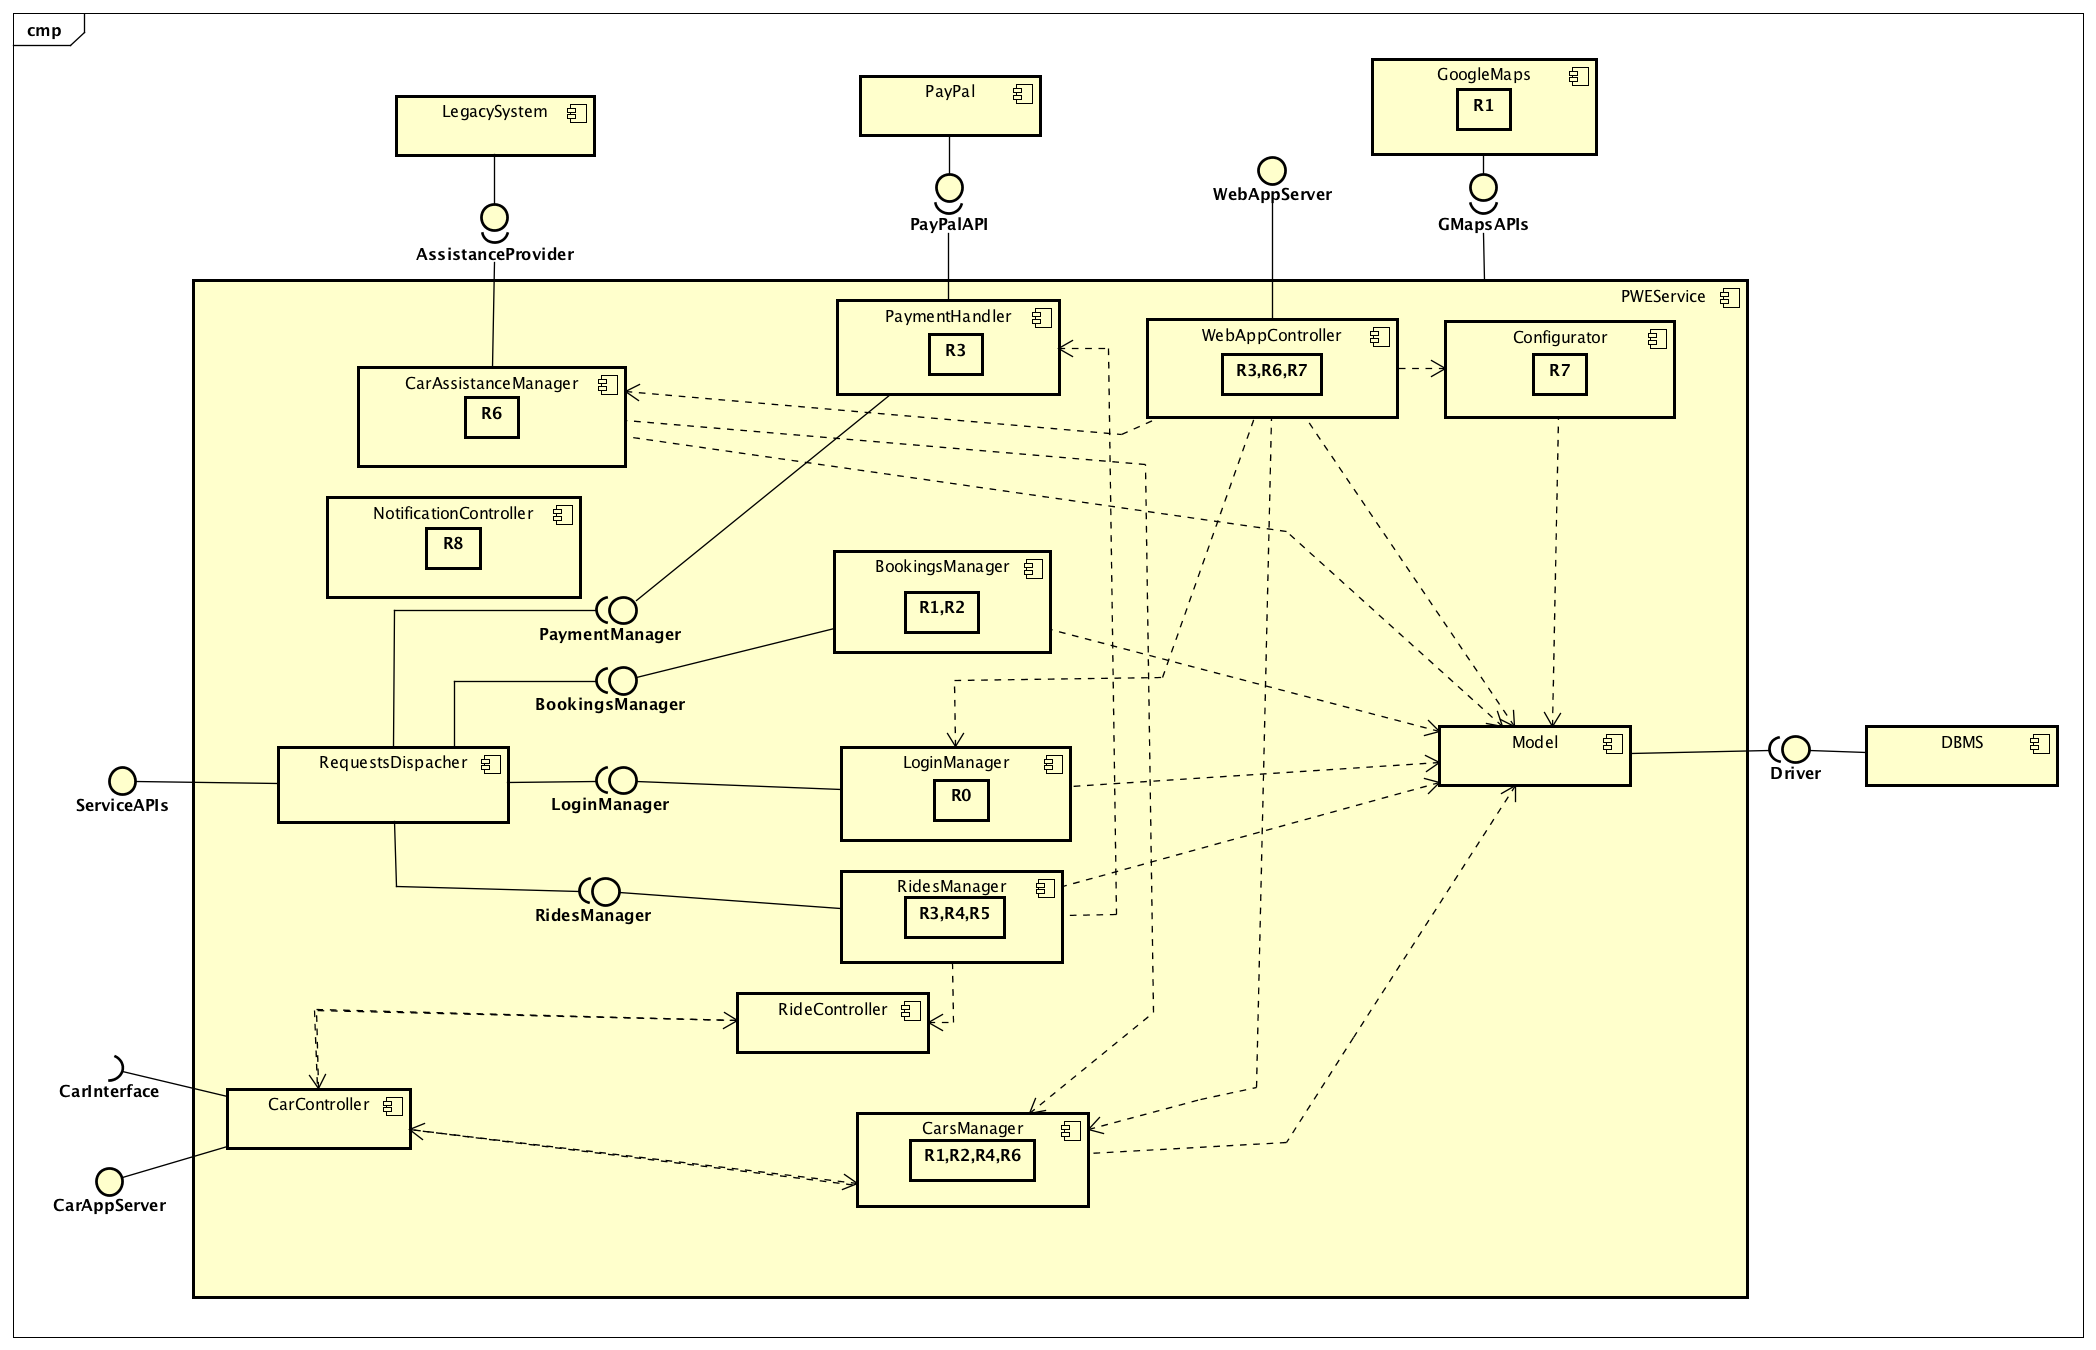
\includegraphics[width=1.00000\textwidth,height=1.00000\textwidth]{./comp_diagrams/system_reqt.png}
\caption{}\label{id}
\end{figure}

\begin{figure}
\centering
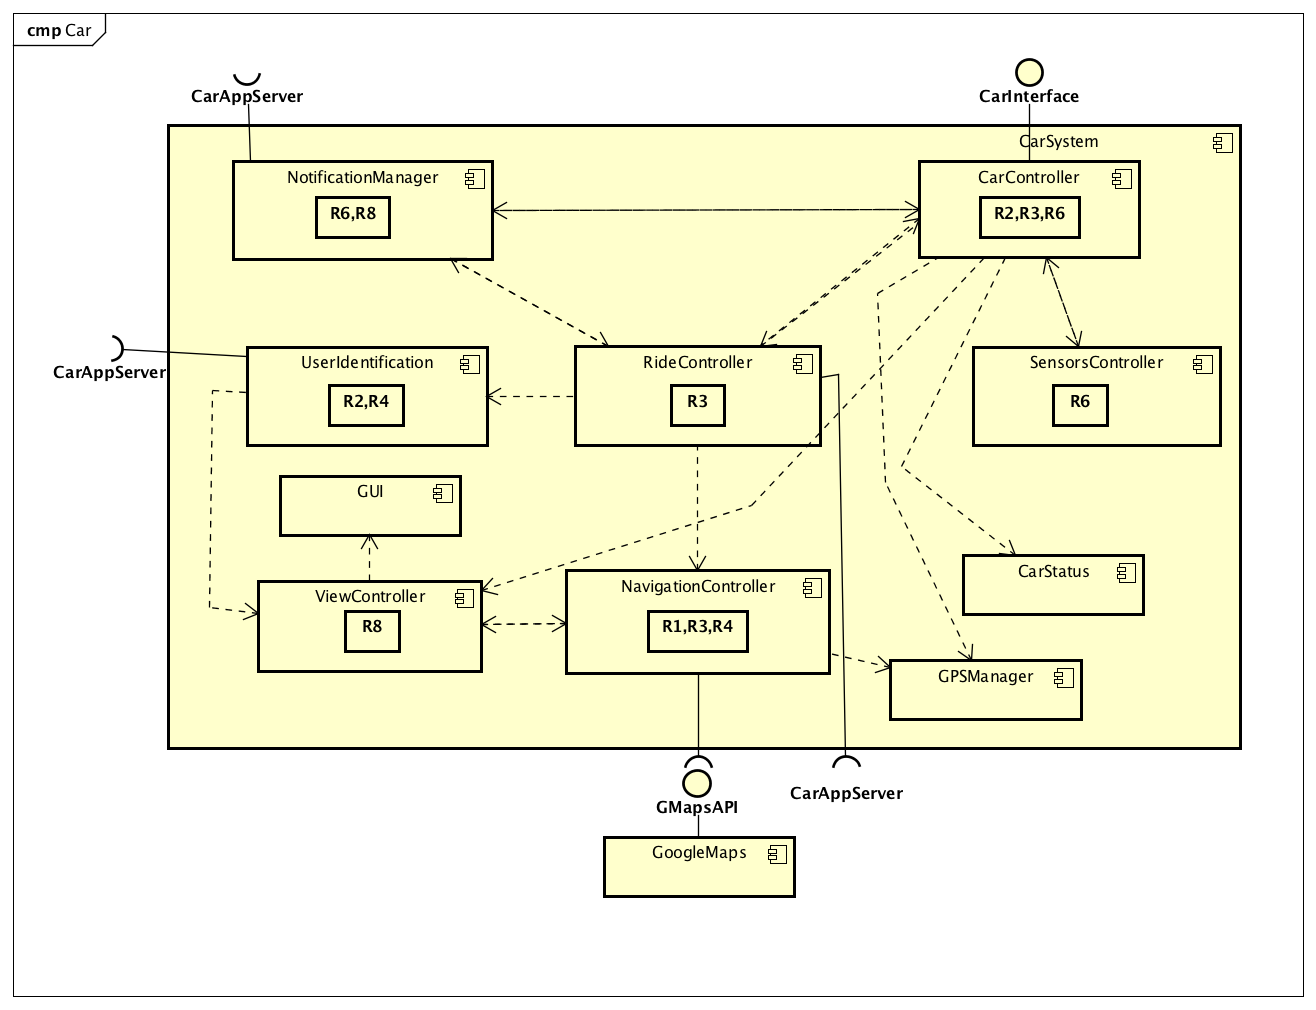
\includegraphics[width=1.00000\textwidth,height=1.00000\textwidth]{./comp_diagrams/car_reqt.png}
\caption{}\label{id}
\end{figure}

How we are going to meet the non-functional requirements will be
clarified in the architectural choices, but in general:

\begin{itemize}
\tightlist
\item
  {[}NFR1{]} We will use Adobe PhoneGap to develop a multi-platform
  application.
\item
  {[}NFR2{]} We will use efficient communication protocols and
  lightweight data formats.
\item
  {[}NFR3{]} Usage of firewalls(as mentioned before) and TLS.
\end{itemize}

\subsection{Architectural and technological
choices}\label{architectural-and-technological-choices}

\begin{figure}
\centering
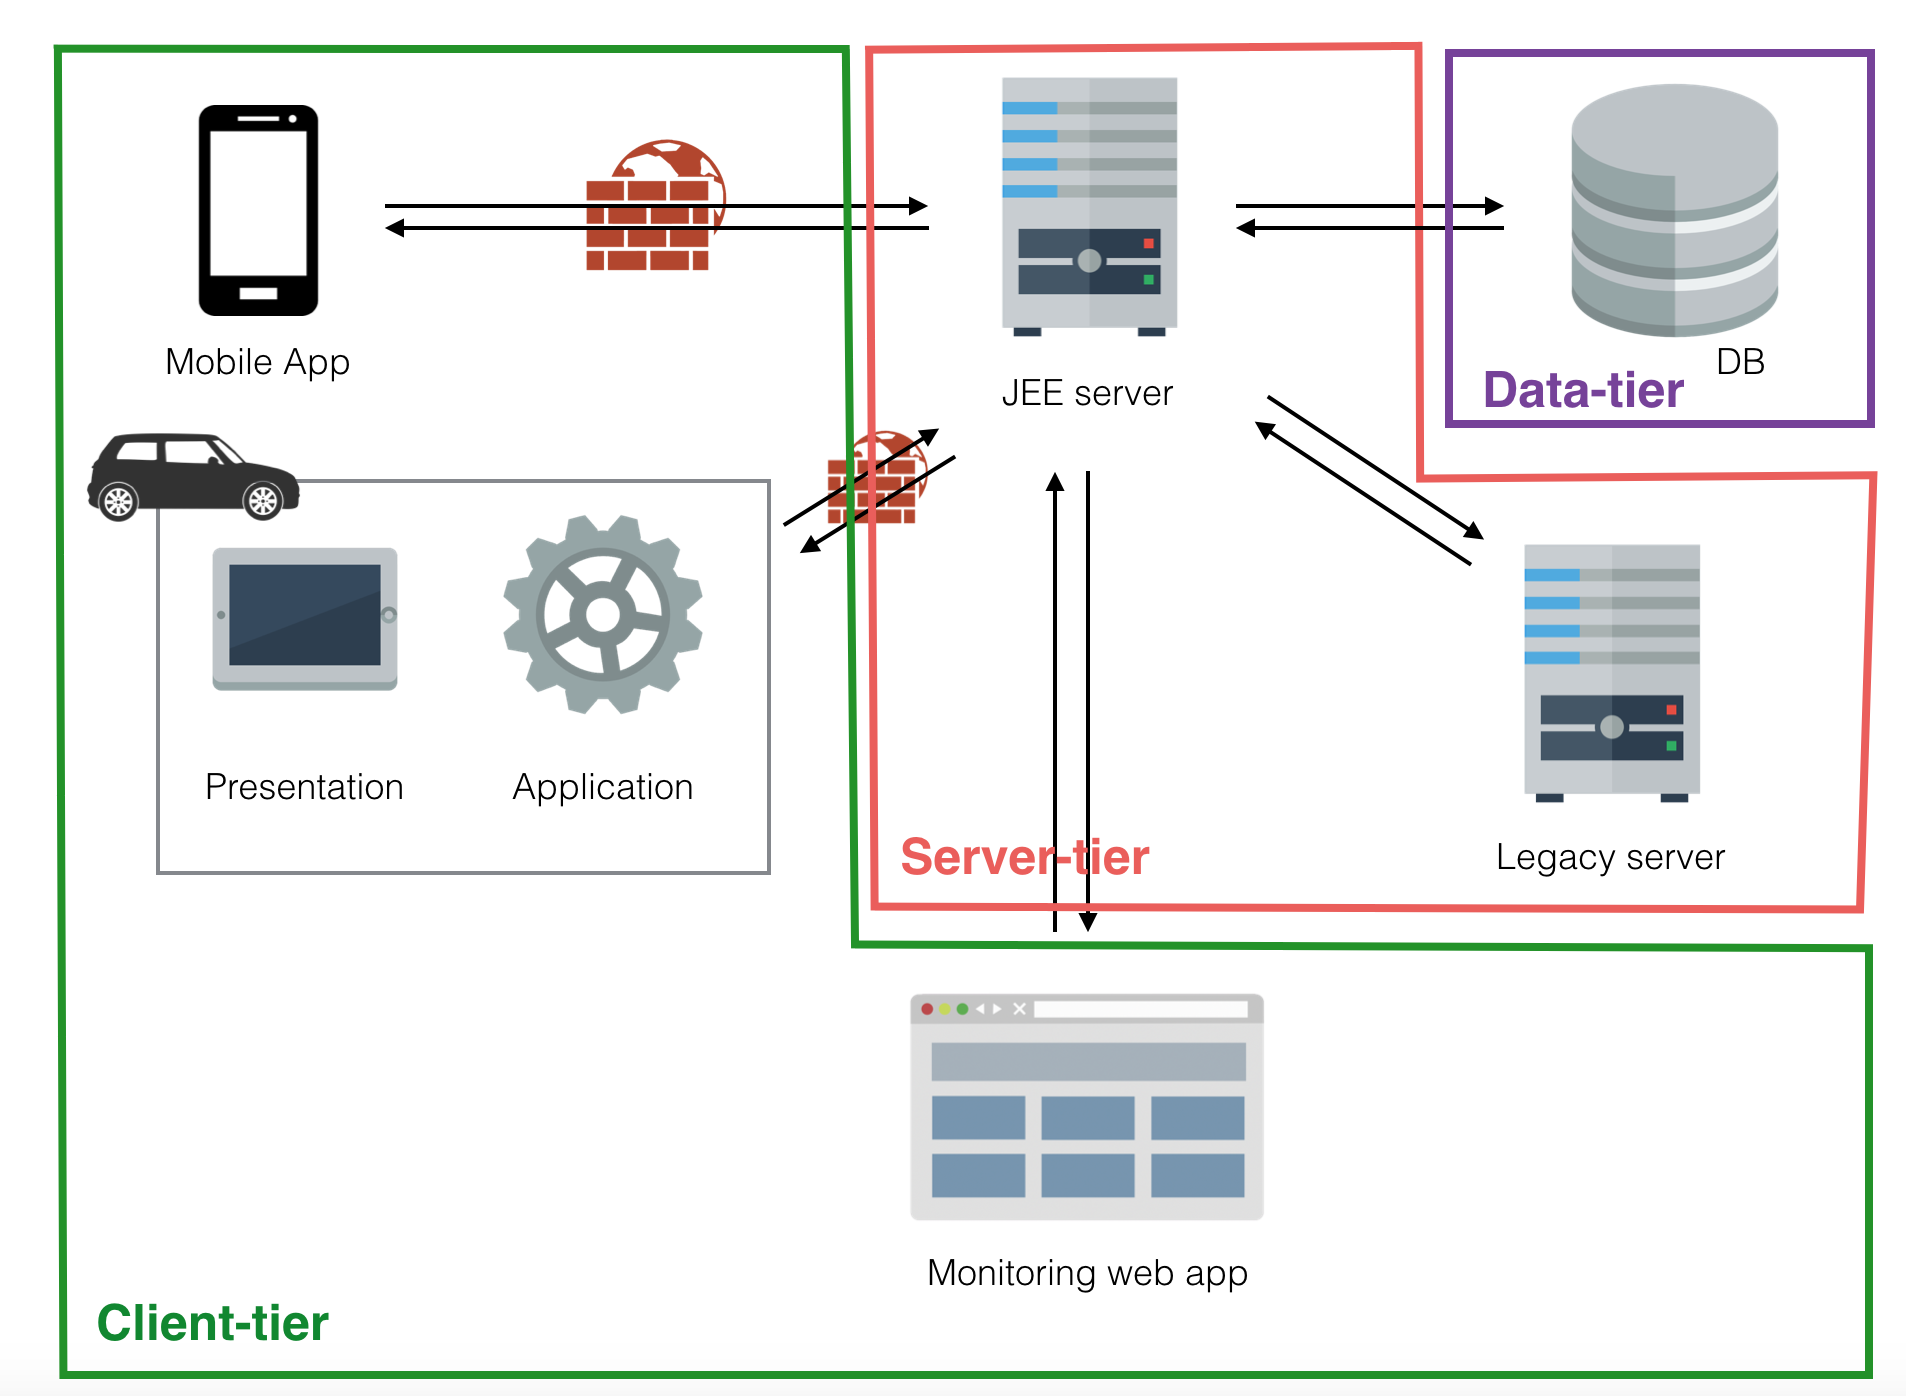
\includegraphics[width=1.00000\textwidth,height=1.00000\textwidth]{./images/sysApp.png}
\caption{}\label{id}
\end{figure}

\subsubsection{Server-side (Web , Business Logic and Data
tiers)}\label{server-side-web-business-logic-and-data-tiers}

\begin{itemize}
\item
  We will develop our application and web server using the Java
  EnterpriseEdition framework (formally, using JEE, we should refer to
  our application as multi-tier, but for simplicity sake and because our
  system is distributed over client machines, JEE server machine and a
  database we will consider it three-tier) .

  \begin{itemize}
  \tightlist
  \item
    JEE will allow us to shorten the development time and to achieve
    high performances while keeping our application complexity
    manageable.
  \item
    JEE makes our project use architectural structure that follows
    well-known best practices.
  \end{itemize}
\item
  We will use Oracle GlassFish Server (the commercial edition) as
  application server.

  \begin{itemize}
  \tightlist
  \item
    GlassFish gives very good performance guarantees and is well
    supported.
  \end{itemize}
\item
  We will use the JAX-RS APIs to expose RESTful APIs with JSON that will
  be used from the mobile app to interface with the web server.

  \begin{itemize}
  \tightlist
  \item
    The usage of the RESTful standard will give our system robustness
    and flexibility.
  \item
    This will allow us to use Adobe PhoneGap to develop an hybrid
    multi-platform application for the client side.
  \item
    The usage of JSON helps with optimizing the usage of bandwidth.
  \end{itemize}
\item
  We will use the MySQL to manage our Database.

  \begin{itemize}
  \tightlist
  \item
    We don't need advanced feature for data management that other DBMSs
    offer.
  \item
    MySQL is fast and easy to use.
  \item
    Free.
  \item
    Compatible with JDBC.\newline
  \end{itemize}
\item
  TLS will be used for confidential information communication.
\end{itemize}

\subsubsection{Client-side}\label{client-side}

\paragraph{Mobile application}\label{mobile-application}

\begin{itemize}
\item
  We will develop our application using the standard web technologies
  (AngularJS, HTML, css) and use Adobe PhoneGap (built on Apache
  Cordova) to create a multi-platform mobile app. This approach will
  allow us to:
\item
  Benefit from the experience of our engineers in web development.
\item
  Reduce development time and cost.\newline
  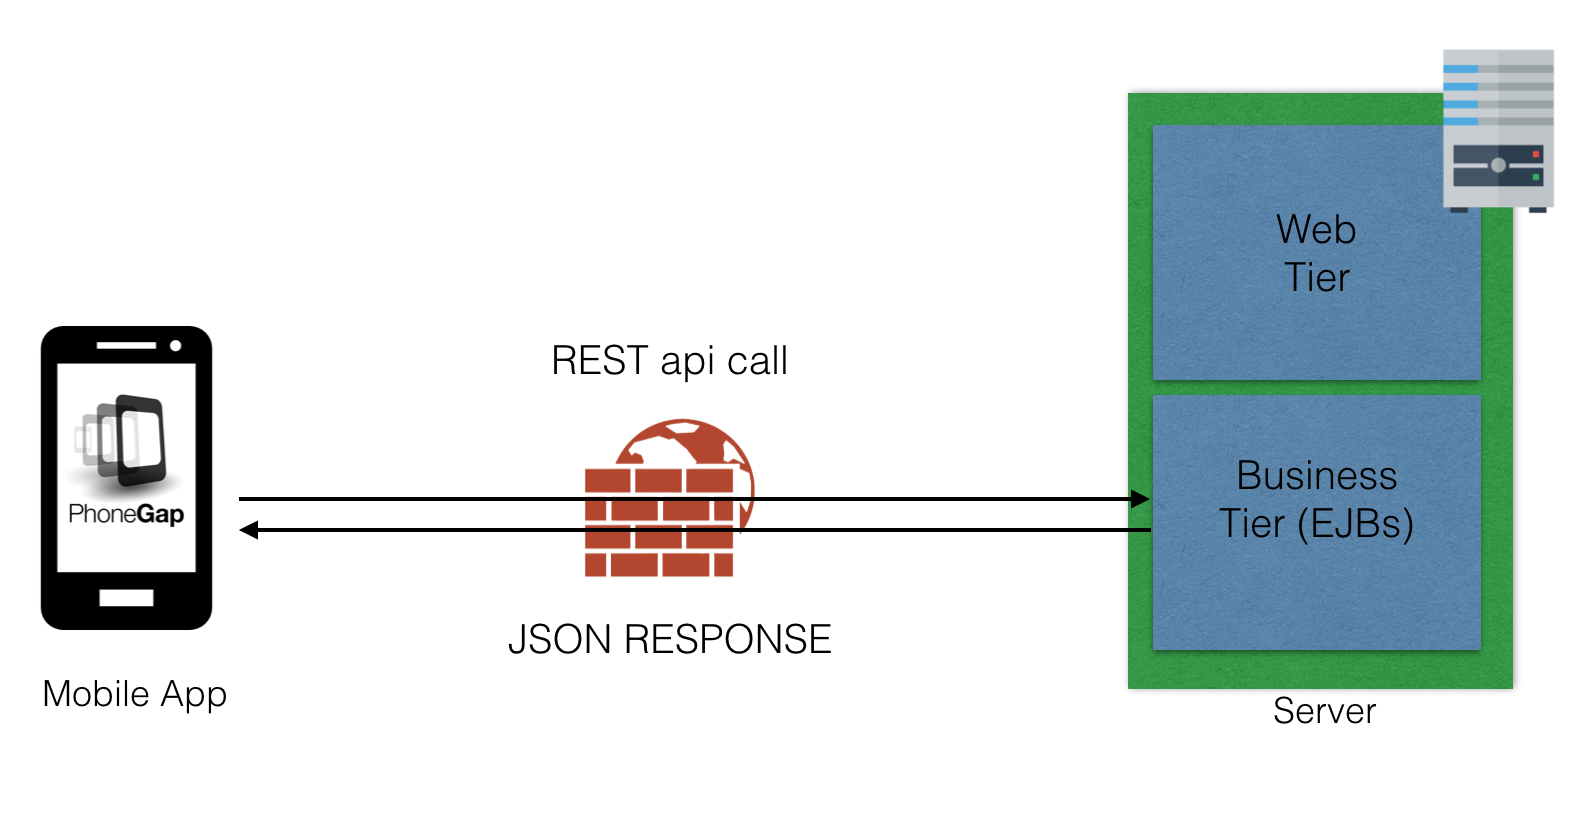
\includegraphics[width=1.00000\textwidth,height=1.00000\textwidth]{./images/appArch.png}
\end{itemize}

\paragraph{Monitoring WebApp}\label{monitoring-webapp}

\begin{itemize}
\item
  We will develop the monitoring Web using a JEE web server exploiting
  the JavaServlet framework.
\item
  Easy to deploy and develop.\newline
  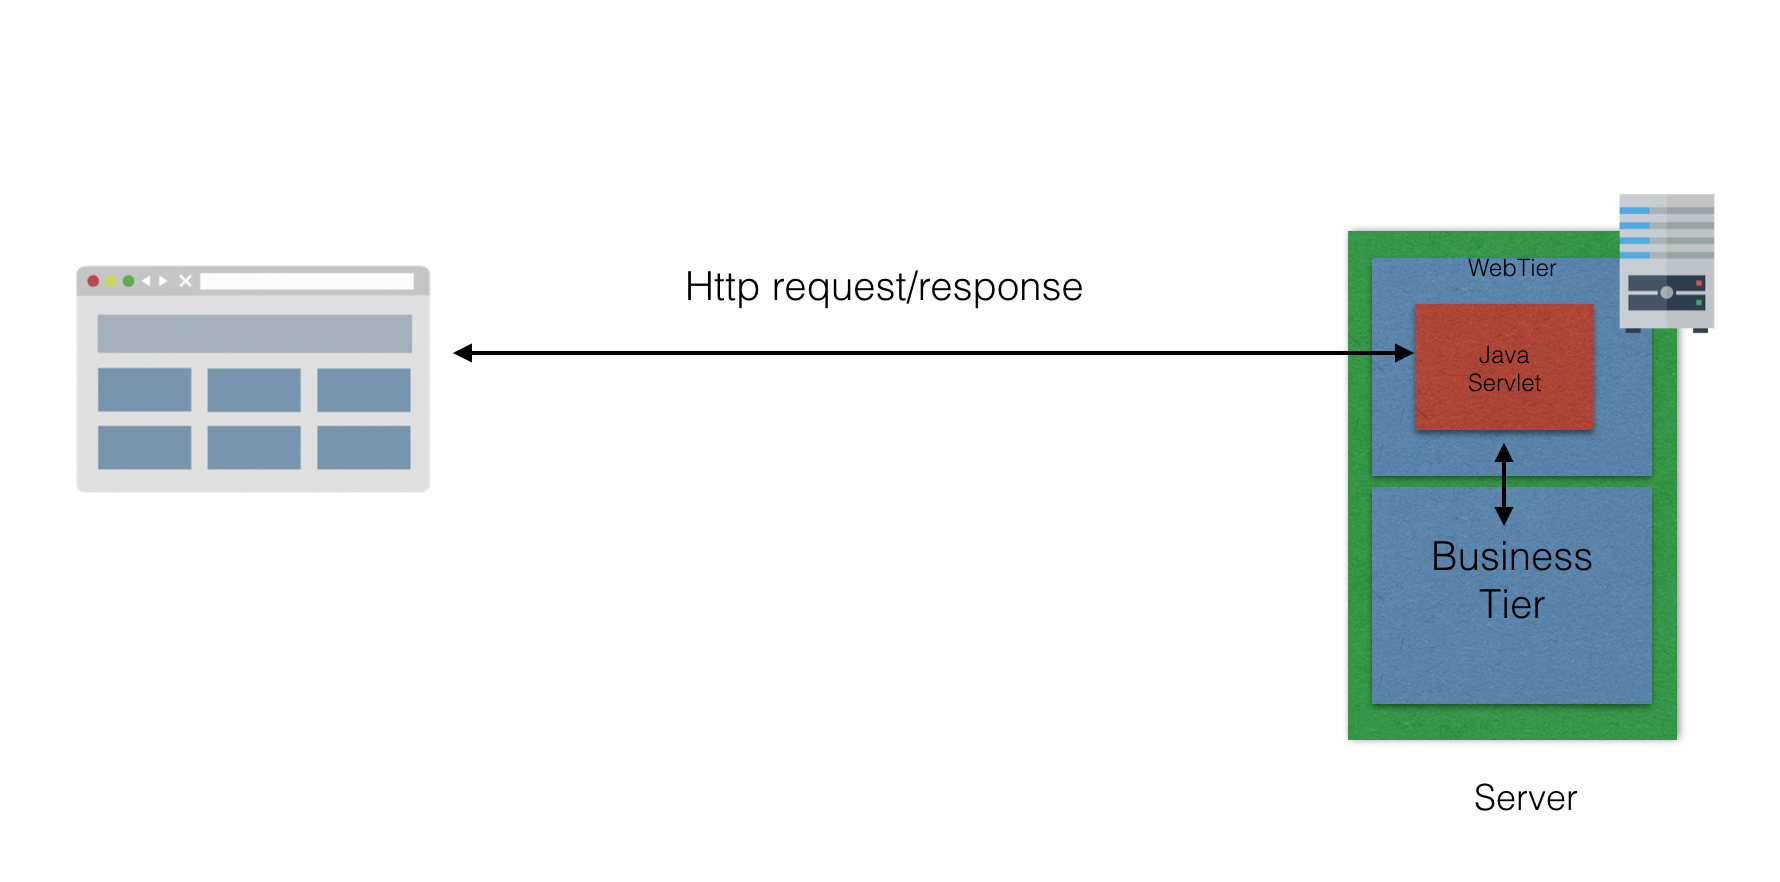
\includegraphics[width=1.00000\textwidth,height=1.00000\textwidth]{./images/webAppArch.png}
\end{itemize}

\paragraph{Car on-board application}\label{car-on-board-application}

\begin{itemize}
\item
  We will develop a Java application to run in the system of the car.
\item
  We need a tool to have control over the car status.
\item
  The application needs to contain not only presentation features, but
  also logic to elaborate the data coming from the sensors and manage
  the execution of a ride without a continuos interaction with the
  server and deal with real time issues.
\item
  The application will be able to retrieve informations from the car
  sensors (such as the battery level or the presence of mechanical
  problems)through OBD connector(Java libraries to read information from
  an OBD adapter already exist).
\item
  For the communication with the server a RemoteProcedureCall approach
  will be used.

  \begin{itemize}
  \tightlist
  \item
    Well supported by JEE.
  \item
    It's intuitive and practical to represent cars as remote objects.
  \end{itemize}
\end{itemize}

\begin{figure}
\centering
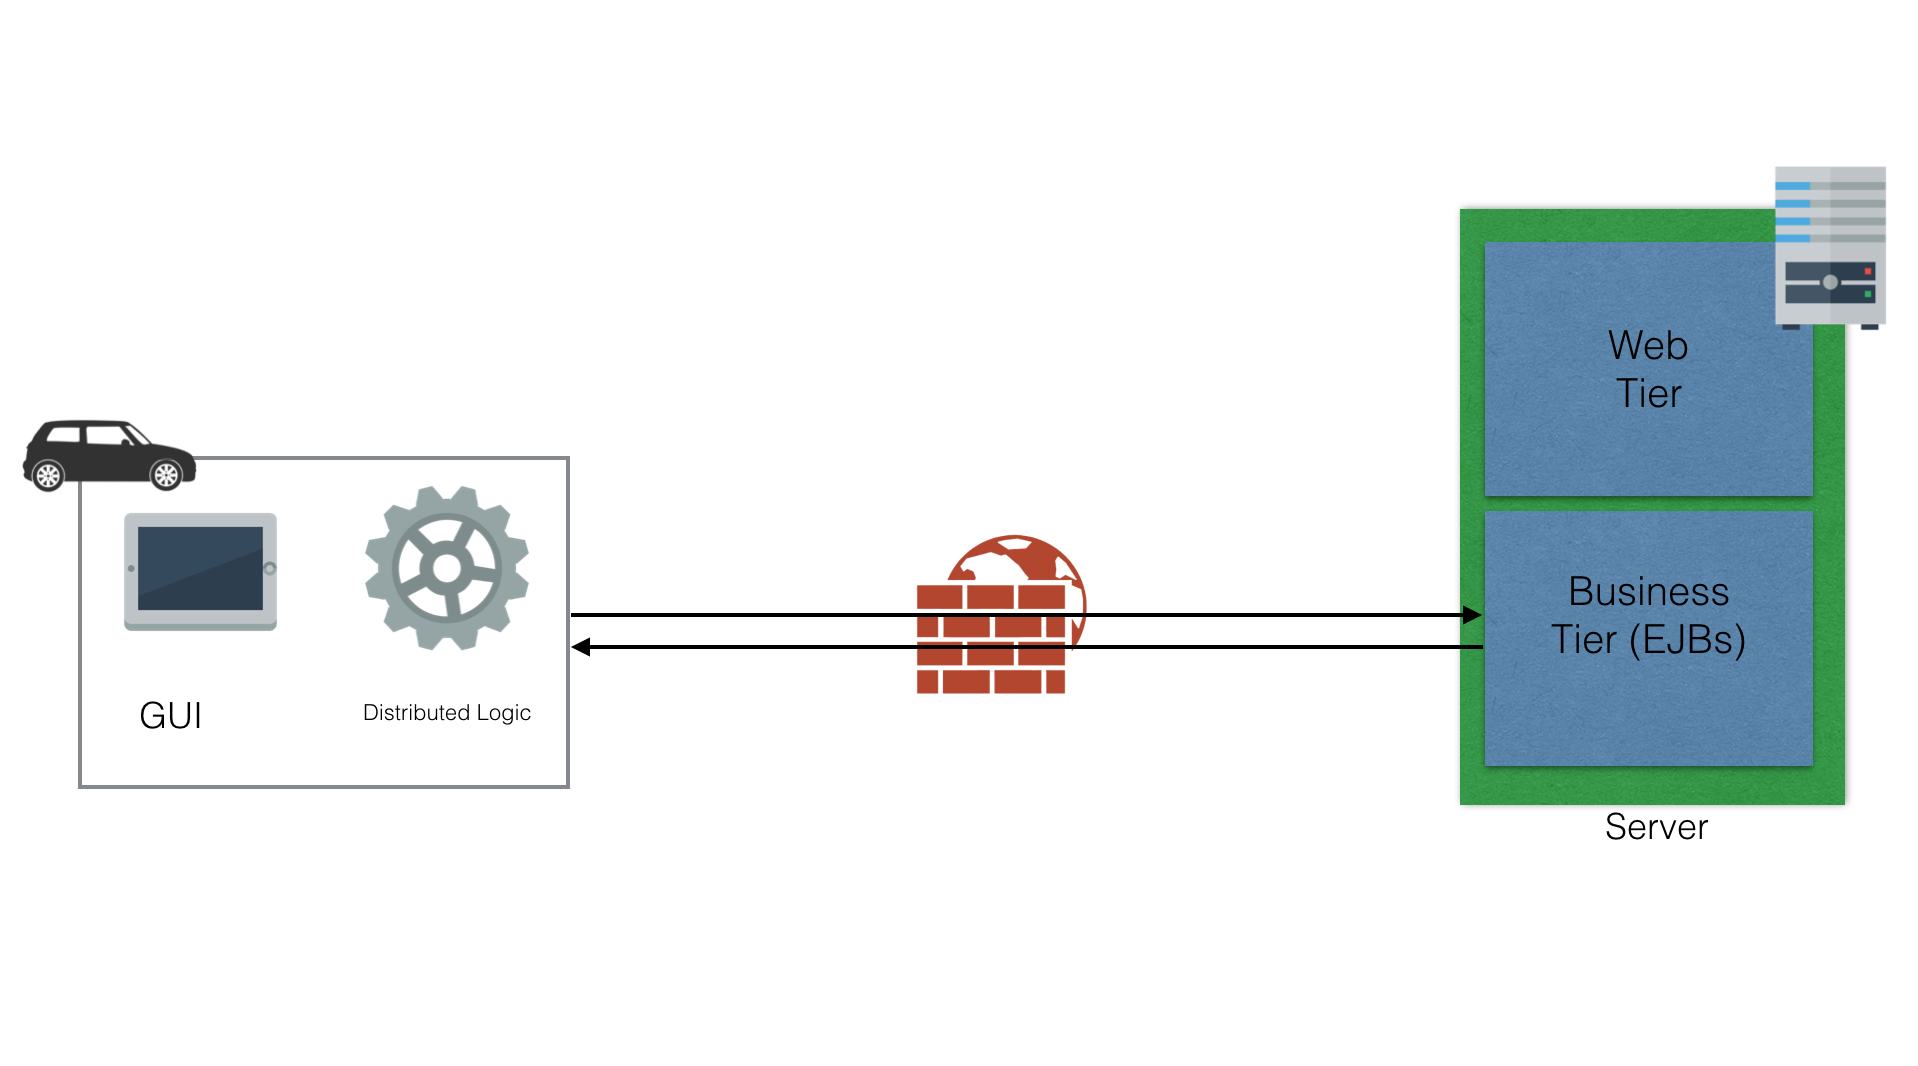
\includegraphics[width=1.00000\textwidth,height=1.00000\textwidth]{./images/carAppArch.png}
\caption{}\label{id}
\end{figure}

\subsection{Patterns}\label{patterns}

These are the main design patterns that we are following in the design
process and many of those are good practices imposed by the adoption of
the JEE framework.

\begin{itemize}
\tightlist
\item
  Model-Control-View : used for almost every component of the system.
  It's a really good choice of design that allows to keep very clear the
  role of every component of the system and that makes the system easy
  to deploy and maintain.
\item
  Client-server : the staple good practice of a web based system.
\end{itemize}

\subsection{Deployment view}\label{deployment-view}

This diagram purpose is to show the hardware components of our system,
and where the code is running.\newline
\centerline{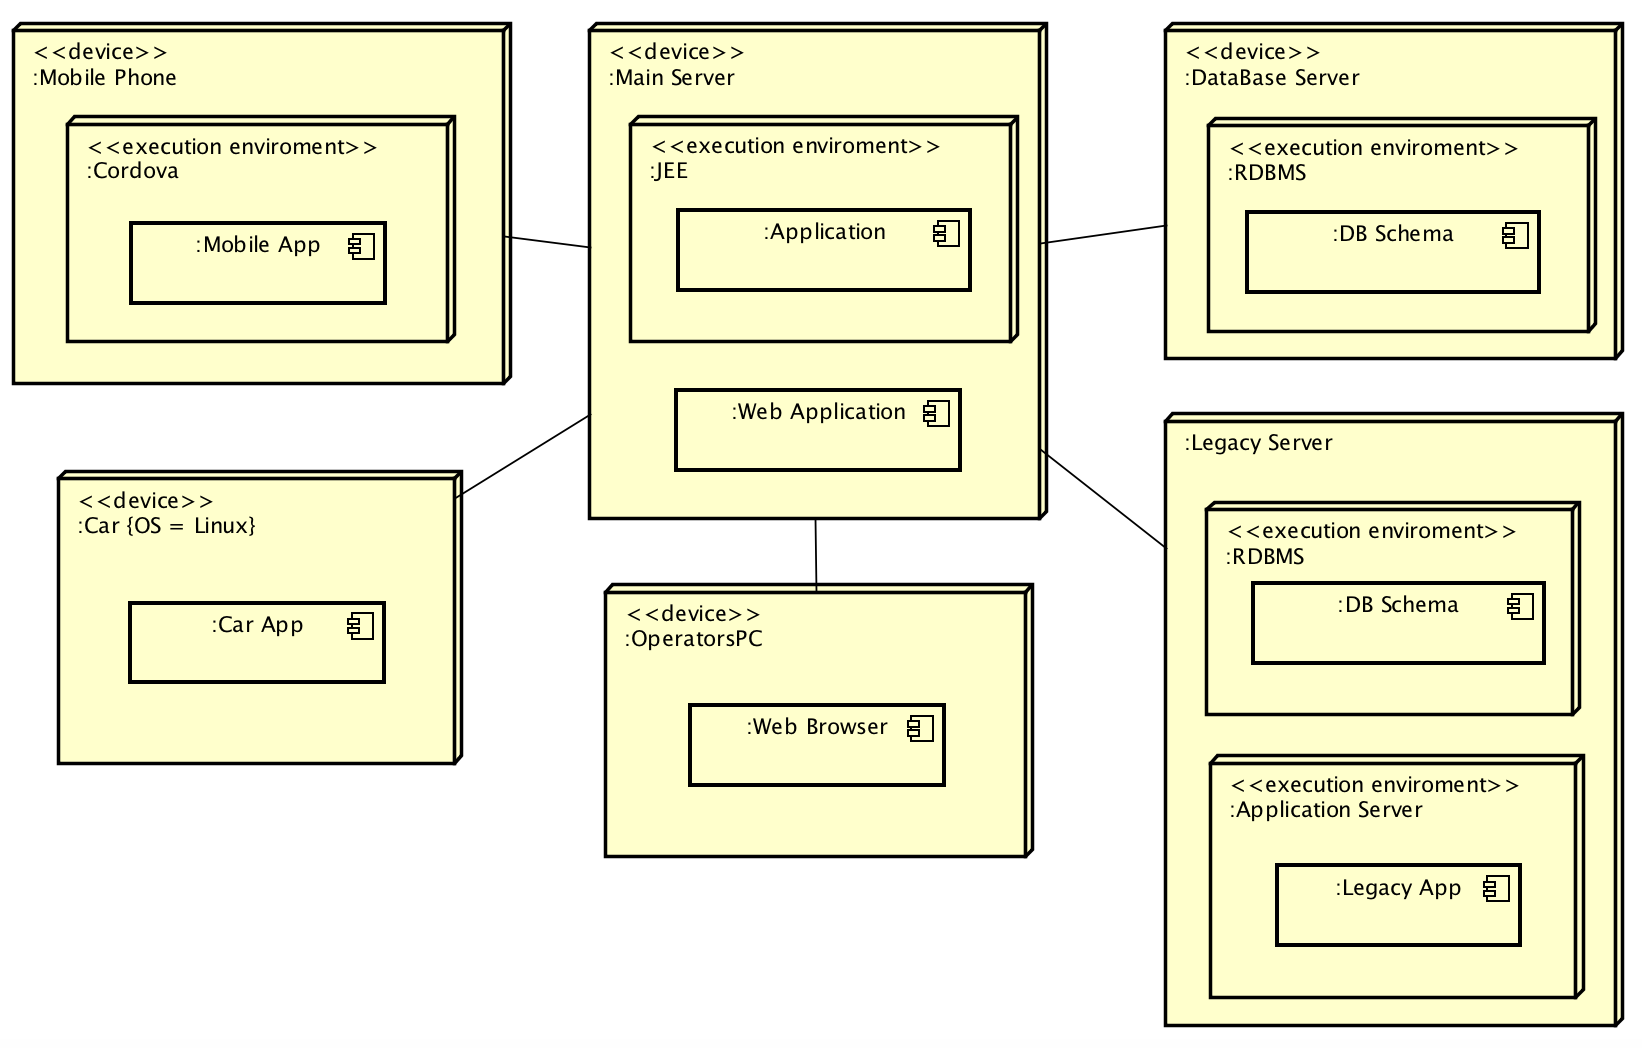
\includegraphics{./deployment/diagram.png}}

\subsection{Runtime view}\label{runtime-view}

\subsection{Component Interfaces}\label{component-interfaces}

\section{Algorithm design}\label{algorithm-design}

\section{User Interface design}\label{user-interface-design}

\subsection{User Experience diagrams}\label{user-experience-diagrams}

These diagrams show how users will interact with the system.

\subsubsection{Mobile application}\label{mobile-application-1}

\centerline{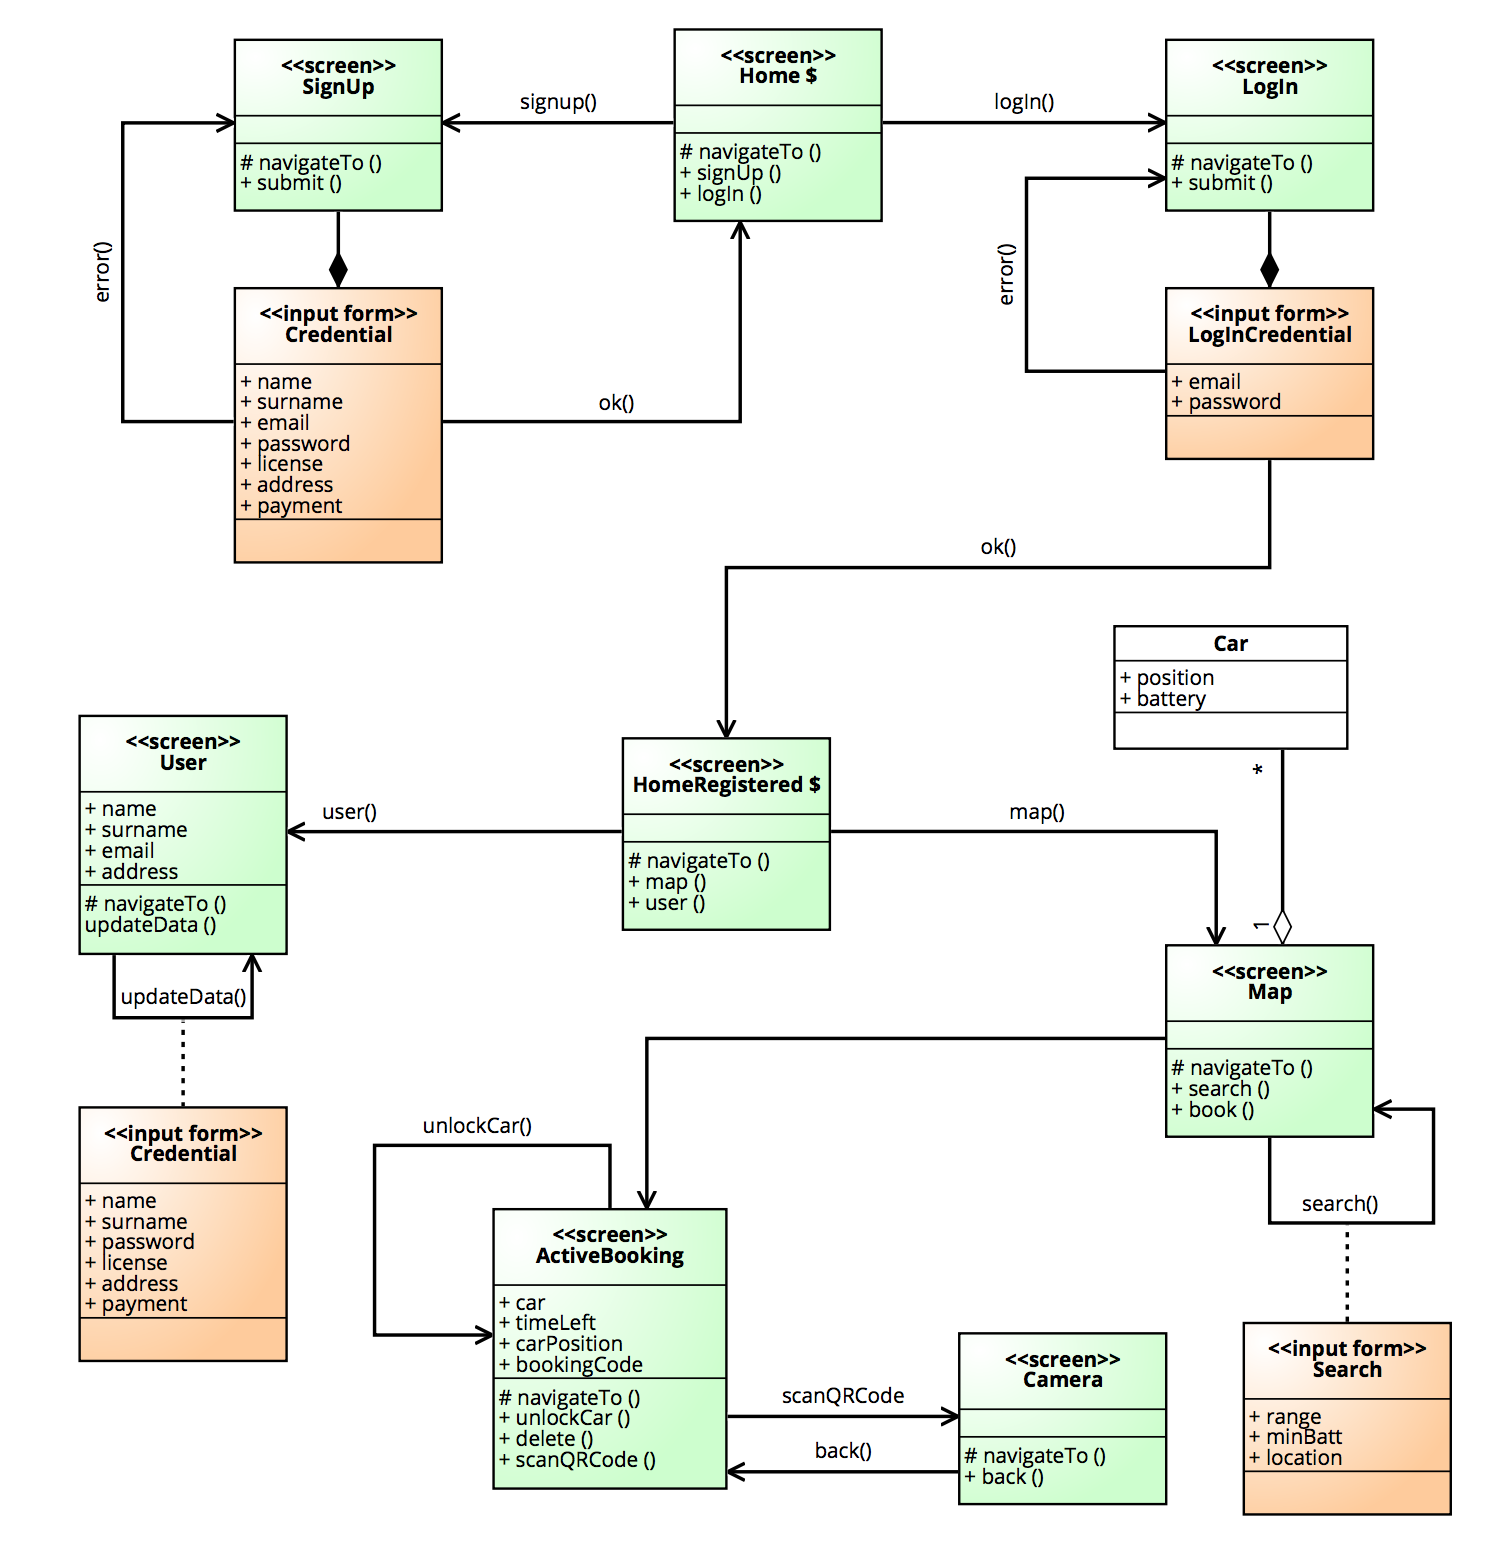
\includegraphics{./images/UX_Mobile.png}}

\subsubsection{Car application}\label{car-application}

\centerline{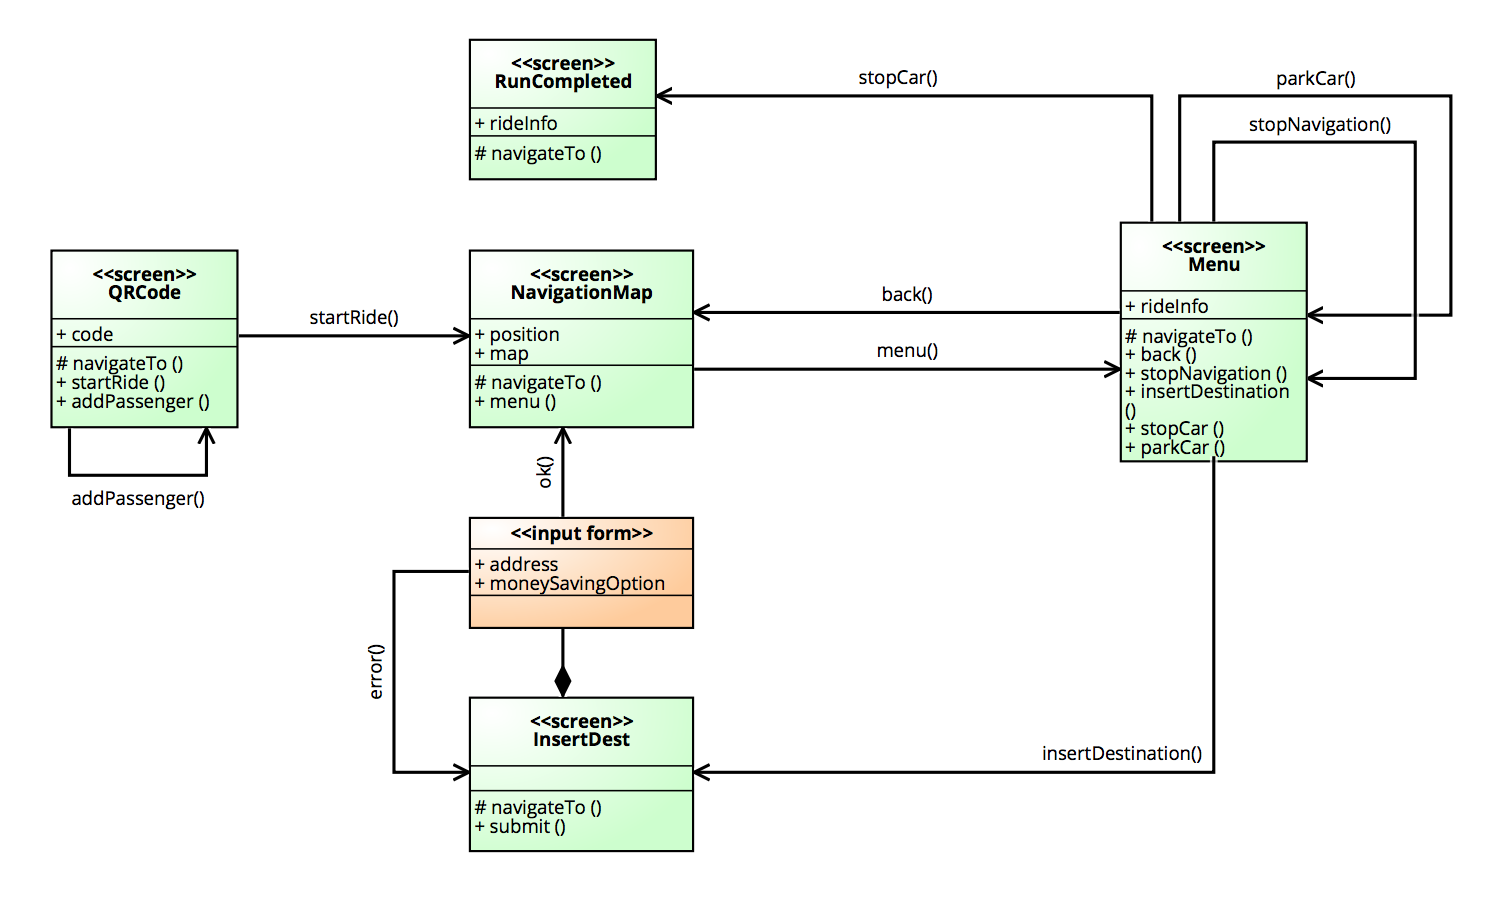
\includegraphics{./images/UX_Car.png}}

\subsubsection{Operators application}\label{operators-application}

\centerline{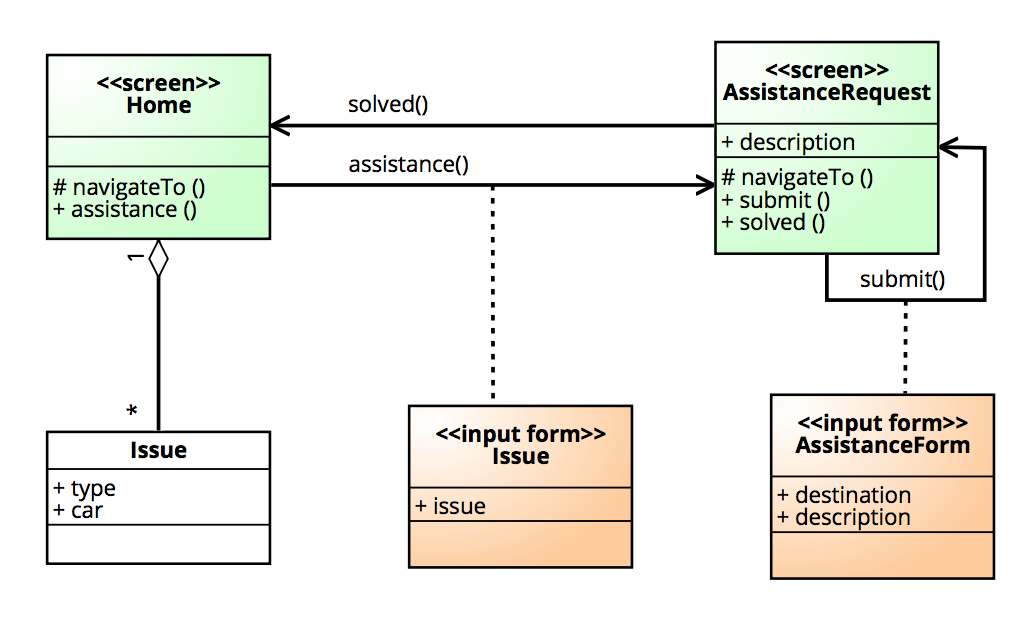
\includegraphics{./images/UX_Operator.png}}

\subsection{Boundary entity control
diagrams}\label{boundary-entity-control-diagrams}

These diagrams are here to show how each action is performed by the
system. The entities representation is simplified to show only the
relevant parts.

\subsubsection{Mobile application}\label{mobile-application-2}

\centerline{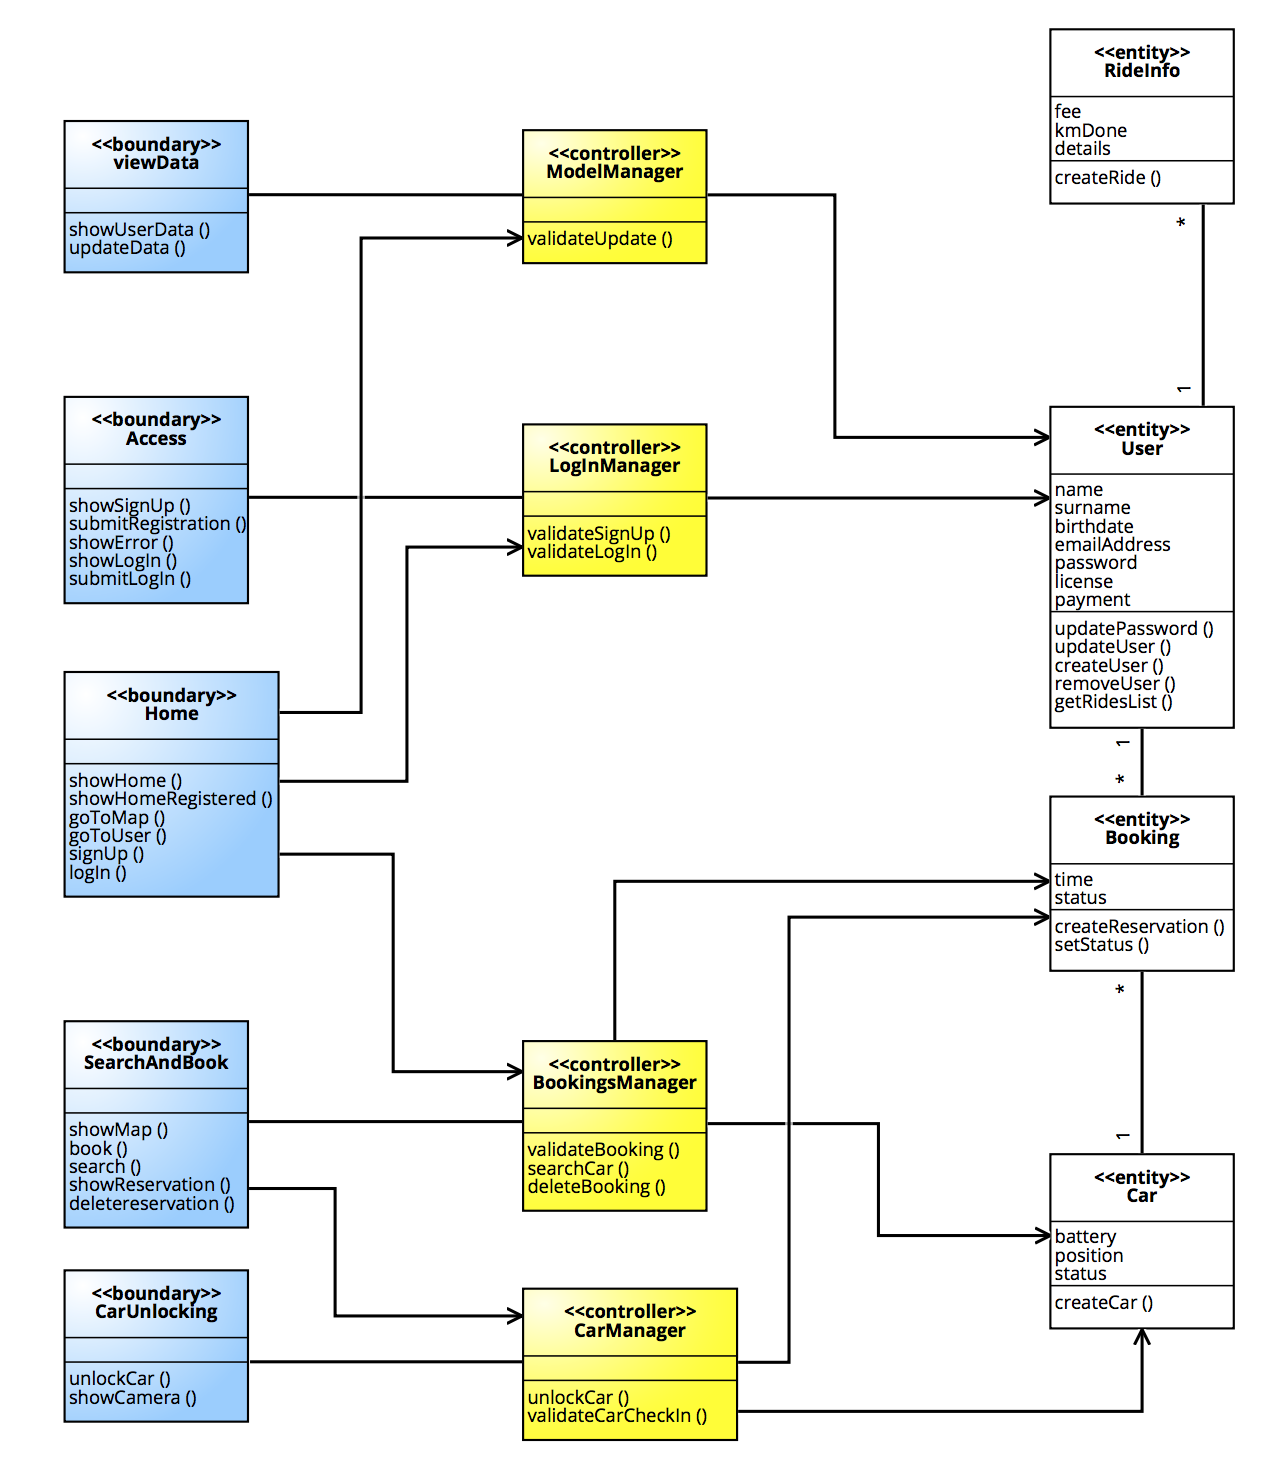
\includegraphics{./images/BCE_Mobile.png}}

\subsubsection{Car application}\label{car-application-1}

\centerline{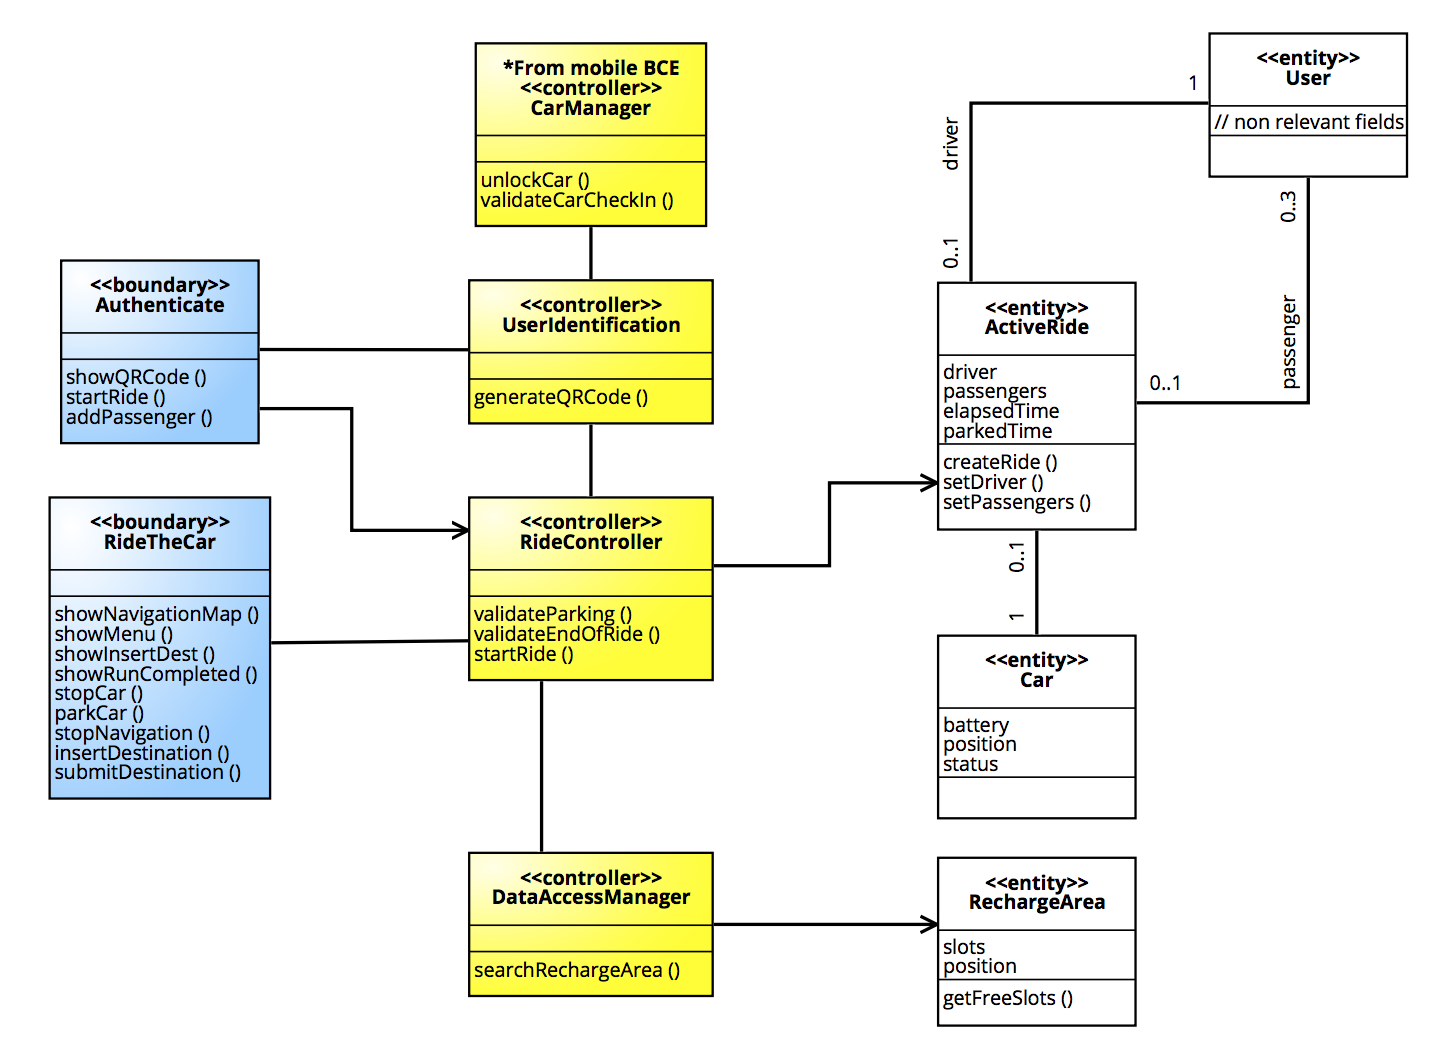
\includegraphics{./images/BCE_Car.png}}

\subsubsection{Operators application}\label{operators-application-1}

\centerline{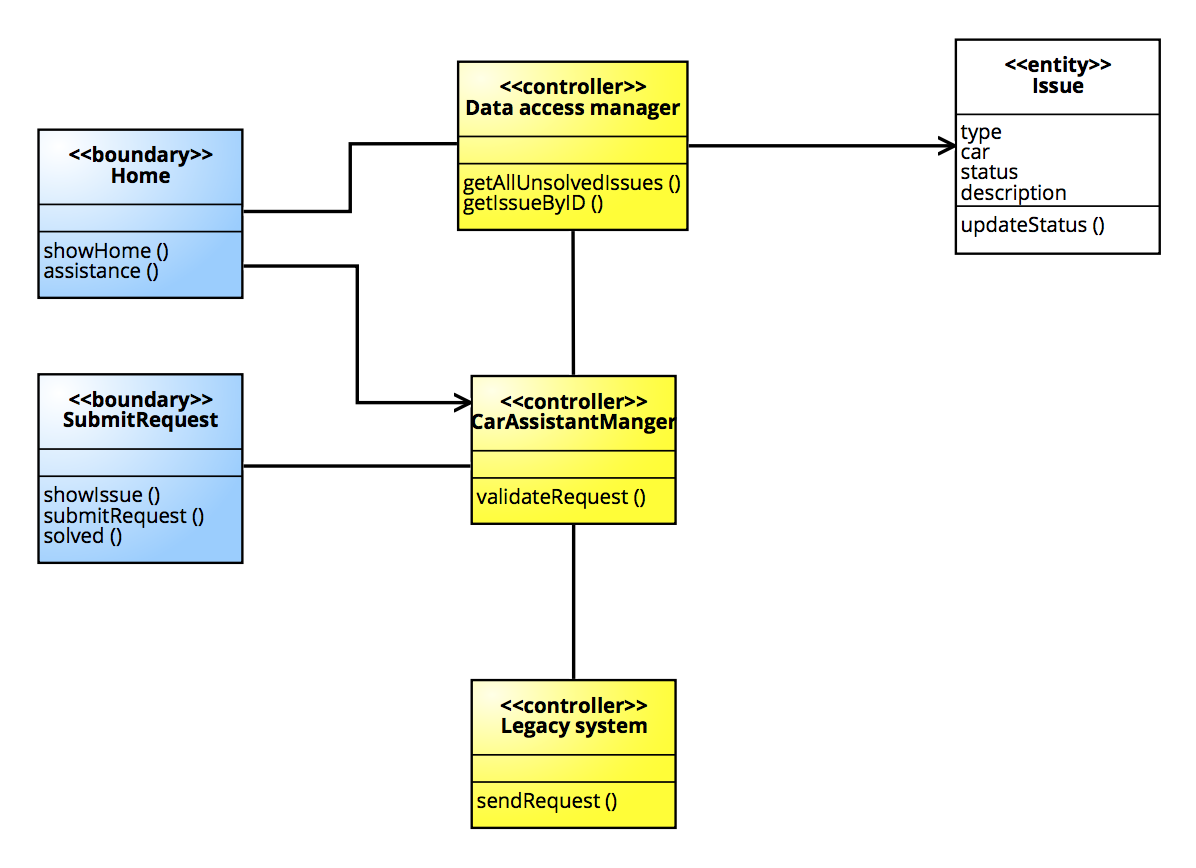
\includegraphics{./images/BCE_Operator.png}}

\section{Effort spent}\label{effort-spent}

\end{document}
